\documentclass[a4paper,12pt]{ctexart} % 使用 ctexart 支持中文

% ------------------- 页面设置 -------------------
\usepackage[left=2.5cm, right=2.5cm, top=2.5cm, bottom=2.5cm]{geometry} % 页边距

% ------------------- 数学宏包 -------------------
\usepackage{amsmath, amssymb, amsfonts, amsthm} % 基础数学包
\usepackage{mathtools} % 数学工具修正
\usepackage{bm}        % 用于加粗向量，例如 \bm{x}

% ------------------- 表格宏包 (运筹学单纯形表必备) -------------------
\usepackage{booktabs}  % 提供 \toprule, \midrule, \bottomrule 等美观横线
\usepackage{multirow}  % 表格单元格合并
\usepackage{array}     % 增强表格功能
\usepackage{longtable} % 长表格（跨页）
\usepackage[hidelinks]{hyperref}

% ------------------- 绘图宏包 (网络流/图论) -------------------
\usepackage{tikz}
\usetikzlibrary{arrows.meta, positioning, shapes, graphs}

% ------------------- 代码/算法伪代码 -------------------
\usepackage{algorithm}
\usepackage{algorithmicx}
\usepackage{algpseudocode}

% ------------------- 自定义环境 -------------------
\newtheorem{definition}{定义}[section]
\newtheorem{theorem}{定理}[section]
\newtheorem{lemma}{引理}[section]
\newtheorem{example}{例题}[section]

% 自定义“解”的环境
\newenvironment{solution}{\begin{proof}[\textbf{解}]}{\end{proof}}

% ------------------- 头部信息 -------------------
\title{\textbf{运筹学考试重点复习笔记}}
\author{Ao Yu}
\date{\today}

% =================== 正文开始 ===================
\begin{document}
	
	\maketitle
	\tableofcontents % 生成目录
	\newpage
	
	% 这里是示例内容，之后我会把图片内容填入类似的结构中
	\section{线性规划 (Linear Programming)}
	
	\subsection{例题 1：加工奶制品的生产计划}
	
	\textbf{问题描述：}
	加工一桶牛奶可以得出两种奶制品 $A_1$ 和 $A_2$。
	\begin{itemize}
		\item 生产 $A_1$：需加工 12 小时，可产出 3 公斤，每公斤获利 24 元。
		\item 生产 $A_2$：需加工 8 小时，可产出 4 公斤，每公斤获利 16 元。
	\end{itemize}
	\textbf{现有资源与限制：}
	每天加工 50 桶牛奶，工作时长为 480 小时。其中奶制品 $A_1$ 最多可生产 100 公斤。
	\textbf{问题：} 怎样制定生产计划，才能使每天获利最大？
	
	% --- 流程图 (对应图片1中的示意图) ---
	\begin{figure}[h]
		\centering
		\begin{tikzpicture}[node distance=1.5cm, auto,
			box/.style={draw, rectangle, align=center, minimum height=2em},
			arrow/.style={-Stealth, thick}]
			
			% 定义节点
			\node[box] (input) {1 桶\\牛奶};
			\node[box, right=2cm of input, yshift=1cm] (process1) {12 小时};
			\node[box, right=0cm of process1] (output1) {3 公斤 $A_1$};
			\node[right=0.5cm of output1] (profit1) {获利 24 元/公斤};
			
			\node[box, right=2cm of input, yshift=-1cm] (process2) {8 小时};
			\node[box, right=0cm of process2] (output2) {4 公斤 $A_2$};
			\node[right=0.5cm of output2] (profit2) {获利 16 元/公斤};
			
			% 连线
			\draw[arrow] (input) -- (process1.west);
			\draw[arrow] (input) -- (process2.west);
			\draw[arrow] (output1) -- (profit1);
			\draw[arrow] (output2) -- (profit2);
			
			% 添加“或”字
			\node[right=0.5cm of input] {或};
			
		\end{tikzpicture}
		\caption{生产流程示意图}
	\end{figure}
	
	\subsection{模型建立步骤}
	
	\subsubsection*{1. 决策变量}
	分别加工 $x_1$、$x_2$ 桶牛奶用于生产奶制品 $A_1$、$A_2$。
	
	\subsubsection*{2. 目标函数}
	\begin{itemize}
		\item 生产 $A_1$ 每天获利：$z_1 = 24 \times 3x_1 = 72x_1$
		\item 生产 $A_2$ 每天获利：$z_2 = 16 \times 4x_2 = 64x_2$
	\end{itemize}
	即每天总获利：
	$$ z = z_1 + z_2 = 72x_1 + 64x_2 $$
	
	\subsubsection*{3. 约束条件}
	\begin{enumerate}
		\item \textbf{原料供应约束} (牛奶桶数)：$x_1 + x_2 \leq 50$
		\item \textbf{劳动时间约束} (加工工时)：$12x_1 + 8x_2 \leq 480$
		\item \textbf{加工能力约束} ($A_1$产量限制)：$3x_1 \leq 100$
		\item \textbf{非负约束}：$x_1, x_2 \geq 0$
	\end{enumerate}
	
	\subsection{最终数学模型}
	
	该问题的数学模型整理如下：
	
	\begin{equation}
		\begin{aligned}
			\max \quad & z = 72x_1 + 64x_2 \\
			\text{s.t.} \quad & \left\{
			\begin{aligned}
				x_1 + x_2 & \leq 50 \\
				12x_1 + 8x_2 & \leq 480 \\
				3x_1 & \leq 100 \\
				x_1, x_2 & \geq 0
			\end{aligned}
			\right.
		\end{aligned}
	\end{equation}
	\subsection{对偶问题 (Dual Problem)}
	
	\textbf{对偶理论简介：}
	对于每一个线性规划的原问题（Primal Problem），都存在一个对偶问题（Dual Problem）。
	\begin{itemize}
		\item 原问题变量 $x_j$ 对应对偶问题的约束。
		\item 原问题约束 $i$ 对应对偶问题的变量 $y_i$（代表第 $i$ 种资源的影子价格）。
		\item 目标函数由“最大化利润”变为“最小化资源价值”。
	\end{itemize}
	
	\textbf{对偶模型构建：}
	
	设 $y_1, y_2, y_3$ 分别为\textbf{原料供应}、\textbf{劳动时间}、\textbf{加工能力}这三个约束条件的对偶变量。
	
	根据对偶规则（$\max \to \min$, $\leq \to \geq$, 矩阵转置）：
	
	\begin{equation}
		\begin{aligned}
			\min \quad & w = 50y_1 + 480y_2 + 100y_3 \\
			\text{s.t.} \quad & \left\{
			\begin{aligned}
				1y_1 + 12y_2 + 3y_3 & \geq 72 \quad (\text{对应 } x_1) \\
				1y_1 + 8y_2 + 0y_3 & \geq 64 \quad (\text{对应 } x_2) \\
				y_1, y_2, y_3 & \geq 0
			\end{aligned}
			\right.
		\end{aligned}
	\end{equation}
	
	\textbf{经济解释：}
	\begin{itemize}
		\item $y_1$：每桶牛奶的潜在价值（影子价格）。
		\item $y_2$：每小时劳动的潜在价值。
		\item $y_3$：每单位加工能力的潜在价值。
		\item 对偶问题的目标是寻找这些资源的最低估值，使得资源总价值不低于生产产品的获利。
	\end{itemize}
	
	\subsection{单纯形法 (Simplex Method)}
	
	\subsubsection{核心思想}
	单纯形法是一种迭代算法，其几何意义是在线性规划问题可行域的\textbf{顶点}中逐步确定最优解。
	\begin{itemize}
		\item \textbf{顶点移动}：若当前的基本可行解（顶点）不是最优的，就从与该顶点相连的边中找到一条使目标函数下降的边，沿此边移动到相邻的顶点。
		\item \textbf{有限终止}：由于顶点数量有限，只要每次移动都使目标函数优化，经过有限次迭代必能找到最优解。
	\end{itemize}
	
	\subsubsection{算法迭代步骤与表格构造}
	
	% --- 为了模仿 PPT 样式，我们需要定义一个新的表格环境或直接调整 ---
	% 提示：如果编译报错说没有 xcolor，请在导言区加 \usepackage[table]{xcolor}
	% 这里我用基础样式模拟，确保不报错，同时尽可能还原结构。
	
	\subsubsection*{1. 初始单纯形表结构 (General Form)}
	根据课件，初始单纯形表的标准构造如下：
	
	\begin{table}[H]
		\centering
		\renewcommand{\arraystretch}{1.5} % 增加行高，让公式不拥挤
		\begin{tabular}{cccc}
			\toprule
			\textbf{基变量} & $\bm{x_B}$ & $\bm{x_N}$ & \textbf{右端项} \\
			\hline
			\textbf{负函数值} & $0$ & $\hat{c}_N = c_N^T - c_B^T B^{-1} N$ & $-c_B^T B^{-1} b (= -f)$ \\
			\hline
			$\bm{x_B}$ & $I$ & $B^{-1}N$ & $B^{-1}b$ \\
			\bottomrule
		\end{tabular}
		\caption{单纯形表的一般形式}
	\end{table}
	
	\subsubsection*{2. 计算实例详解}
	\textbf{问题标准化}：
	\begin{equation}
		\min \quad z = -2x_1 - 3x_2 \quad \text{s.t.} \quad 
		\begin{cases} 
			-x_1 + x_2 + x_3 = 3 \\ 
			-2x_1 + x_2 + x_4 = 2 \\ 
			4x_1 + x_2 + x_5 = 16 \\ 
			x_1, \dots, x_5 \ge 0 
		\end{cases}
	\end{equation}
	
	\textbf{Step 1: 初始单纯形表}
	
	\begin{table}[H]
		\centering
		\renewcommand{\arraystretch}{1.3}
		\begin{tabular}{c|ccccc|c}
			\toprule
			\textbf{基变量} & $x_1$ & $x_2$ & $x_3$ & $x_4$ & $x_5$ & \textbf{右端项} \\
			\hline
			$-f$ & $-2$ & \textcolor{red}{\textbf{-3}} & $0$ & $0$ & $0$ & $0$ \\
			\hline
			$x_3$ & $-1$ & $1$ & $1$ & $0$ & $0$ & $3$ \\
			$x_4$ & $-2$ & $1$ & $0$ & $1$ & $0$ & $2$ \\
			$x_5$ & $4$ & $1$ & $0$ & $0$ & $1$ & $16$ \\
			\bottomrule
		\end{tabular}
	\end{table}
	
	\textbf{迭代逻辑分析}:
	\begin{itemize}
		\item \textbf{确定入基变量}：由于 $c_2 = -3$ 为绝对值最大的负数，故选择 \textbf{$x_2$} 入基。
		\item \textbf{确定出基变量}：计算最小比值 $\theta$。
		\[ \theta = \min \left\{ \frac{3}{1}, \frac{2}{1}, \frac{16}{1} \right\} = 2 \]
		对应 $x_4$ 行，故 \textbf{$x_4$} 出基。
	\end{itemize}
	
	\textbf{Step 2: 第一次迭代}
	以 $x_2$ 列、 $x_4$ 行的元素（主元 1）为中心进行高斯消元：
	
	\begin{table}[H]
		\centering
		\renewcommand{\arraystretch}{1.3}
		\begin{tabular}{c|ccccc|c}
			\toprule
			\textbf{基变量} & $x_1$ & $x_2$ & $x_3$ & $x_4$ & $x_5$ & \textbf{右端项} \\
			\hline
			$-f$ & \textcolor{red}{\textbf{-8}} & $0$ & $0$ & $3$ & $0$ & $6$ \\
			\hline
			$x_3$ & $1$ & $0$ & $1$ & $-1$ & $0$ & $1$ \\
			$x_2$ & $-2$ & $1$ & $0$ & $1$ & $0$ & $2$ \\
			$x_5$ & $6$ & $0$ & $0$ & $-1$ & $1$ & $14$ \\
			\bottomrule
		\end{tabular}
	\end{table}
	
	\textbf{分析}：$x_1$ 检验数为 $-8 < 0$，非最优。
	\begin{itemize}
		\item \textbf{入基}：\textbf{$x_1$}。
		\item \textbf{出基}：比值 $\min\{1/1, 14/6\}$，选择 \textbf{$x_3$} 出基。
	\end{itemize}
	
	\textbf{Step 3: 第二次迭代}
	以 $x_1$ 列、$x_3$ 行的元素（主元 1）进行消元：
	
	\begin{table}[H]
		\centering
		\renewcommand{\arraystretch}{1.3}
		\begin{tabular}{c|ccccc|c}
			\toprule
			\textbf{基变量} & $x_1$ & $x_2$ & $x_3$ & $x_4$ & $x_5$ & \textbf{右端项} \\
			\hline
			$-f$ & $0$ & $0$ & $8$ & \textcolor{red}{\textbf{-5}} & $0$ & $14$ \\
			\hline
			$x_1$ & $1$ & $0$ & $1$ & $-1$ & $0$ & $1$ \\
			$x_2$ & $0$ & $1$ & $2$ & $-1$ & $0$ & $4$ \\
			$x_5$ & $0$ & $0$ & $-6$ & $5$ & $1$ & $8$ \\
			\bottomrule
		\end{tabular}
	\end{table}
	
	\textbf{分析}：
	检查 $-f$ 行，变量 $x_4$ 的检验数为 $-5 < 0$，说明当前解仍非最优，需继续迭代。
	\begin{itemize}
		\item \textbf{入基}：选择检验数为负的 \textbf{$x_4$}。
		\item \textbf{出基}：计算比值 $\theta$（仅针对系数 $>0$ 的行）。
		$x_1, x_2$ 行系数均为 $-1$，不参与计算；$x_5$ 行系数为 5，比值为 $8/5 = 1.6$。
		故选择 \textbf{$x_5$} 出基。
	\end{itemize}
	
	\textbf{Step 4: 最终迭代（最优表）}
	以 $x_4$ 列、$x_5$ 行的元素（主元 5）为中心进行旋转运算：
	
	\begin{table}[H]
		\centering
		\renewcommand{\arraystretch}{1.3}
		\begin{tabular}{c|ccccc|c}
			\toprule
			\textbf{基变量} & $x_1$ & $x_2$ & $x_3$ & $x_4$ & $x_5$ & \textbf{右端项} \\
			\hline
			$-f$ & $0$ & $0$ & $2$ & $0$ & $1$ & $22$ \\
			\hline
			$x_1$ & $1$ & $0$ & $-0.2$ & $0$ & $0.2$ & $2.6$ \\
			$x_2$ & $0$ & $1$ & $0.8$ & $0$ & $0.2$ & $5.6$ \\
			$x_4$ & $0$ & $0$ & $-1.2$ & $1$ & $0.2$ & $1.6$ \\
			\bottomrule
		\end{tabular}
	\end{table}
	
	\textbf{计算结果}：
	此时 $-f$ 行所有检验数均 $\ge 0$，迭代结束。
	\begin{itemize}
		\item \textbf{最优解}：$x_1=2.6, \quad x_2=5.6, \quad x_4=1.6, \quad x_3=x_5=0$。
		\item \textbf{最优目标函数值}：$z = -22$。
	\end{itemize}
	
	\subsection{内点法 (Interior Point Method) （了解）}
	\textit{注：适用于大规模问题，核心是“从可行域内部逼近最优解”。}
	
	\subsubsection*{核心思想：障碍函数 (Barrier Function)}
	将约束条件 $x_i \geq 0$ 转化为目标函数中的惩罚项（对数障碍函数）：
	$$ \min \quad B(x, \mu) = \bm{c}^T \bm{x} - \mu \sum_{j=1}^{n} \ln(x_j) \quad \text{s.t.} \quad \bm{A}\bm{x} = \bm{b} $$
	其中 $\mu > 0$ 是障碍参数。
	
	\subsubsection*{计算流程}
	\begin{enumerate}
		\item \textbf{初始化}：选择严格在可行域内部的初始点 $\bm{x}^{(0)} > 0$，设定初始 $\mu$ 和缩减因子 $\beta \in (0, 1)$。
		\item \textbf{牛顿迭代方向}：
		对于给定的 $\mu$，利用牛顿法求解 KKT 方程组，得到搜索方向 $d_x$。需要求解如下线性方程组：
		$$
		\begin{bmatrix}
			\bm{S}^{-2} & \bm{A}^T \\
			\bm{A} & \bm{0}
		\end{bmatrix}
		\begin{bmatrix}
			\Delta \bm{x} \\
			\Delta \bm{y}
		\end{bmatrix}
		=
		\begin{bmatrix}
			-\bm{c} + \mu \bm{X}^{-1} \bm{e} \\
			\bm{0}
		\end{bmatrix}
		$$
		(其中 $\bm{X}$ 是对角阵，$\bm{S}$ 是松弛变量对角阵)。
		\item \textbf{更新步长}：
		更新 $\bm{x}^{(k+1)} = \bm{x}^{(k)} + \alpha d_x$，保证新的点仍然在可行域内部（$x > 0$）。
		\item \textbf{收缩 $\mu$}：
		令 $\mu := \beta \mu$，当 $\mu \to 0$ 时，解收敛于原问题的最优解。
	\end{enumerate}
	
	\subsection{梯度下降法 (Gradient Descent) （了解）}
	\textit{注：梯度下降通常用于无约束非线性规划。对于线性规划，由于目标函数梯度是常数且有约束，直接使用较少，通常采用“投影梯度法”。}
	
	\subsubsection*{计算流程}
	\begin{enumerate}
		\item \textbf{计算梯度}：
		对于目标函数 $f(\bm{x}) = \bm{c}^T \bm{x}$，其梯度为常向量 $\nabla f = \bm{c}$。
		\item \textbf{负梯度方向}：
		为了最小化目标函数，应沿着负梯度方向 $-\bm{c}$ 移动。
		\item \textbf{投影 (Projection)}：
		由于线性规划有约束 $\bm{A}\bm{x}=\bm{b}, \bm{x} \geq 0$，直接移动会通过边界。
		计算移动方向 $\bm{d}$，使其是 $-\bm{c}$ 在约束面上的投影：
		$$ \bm{d} = - (\bm{I} - \bm{A}^T(\bm{A}\bm{A}^T)^{-1}\bm{A}) \bm{c} $$
		\item \textbf{确定步长}：
		沿方向 $\bm{d}$ 移动，直到碰到边界（即某个 $x_j$ 变为 0）。
		$$ \bm{x}^{(k+1)} = \bm{x}^{(k)} + \alpha \bm{d} $$
		\item \textbf{迭代}：
		在新的边界上重复投影和移动，直到找不到使目标函数下降的可行方向。
	\end{enumerate}
	
	
	\section{整数规划 (Integer Linear Programming)}
	
	\subsection{基本定义与形式}
	
	整数规划是指决策变量被限制为整数的线性规划问题。
	\begin{itemize}
		\item \textbf{纯整数规划}：所有决策变量要求为整数。
		\item \textbf{混合整数规划 (MIP)}：部分变量要求为整数。
		\item \textbf{0-1 整数规划}：变量 $x_j$ 仅取 0 或 1。
	\end{itemize}
	
	\textbf{数学模型一般形式：}
	\begin{equation}
		\begin{aligned}
			\min \quad & Z = \sum_{j=1}^{n} c_j x_j \\
			\text{s.t.} \quad & \left\{
			\begin{aligned}
				\sum_{j=1}^{n} a_{ij} x_j &= b_i \quad (i = 1, 2, \dots, m) \\
				x_j &\ge 0 \\
				x_j & \in \mathbb{Z} \quad (\text{部分或全部})
			\end{aligned}
			\right.
		\end{aligned}
	\end{equation}
	
	\subsection{建模小技巧 (Tips：0-1 变量的神奇用法)}
	
	在 0-1 规划中，设 $x_i = 1$ 表示选择项目 $i$， $x_i = 0$ 表示不选。
	
	\begin{enumerate}
		\item \textbf{互斥约束 (Mutually Exclusive)}：
		\begin{itemize}
			\item 若项目 A 和 B 中\textbf{至多}选一个：$x_A + x_B \le 1$
			\item 若项目 A 和 B 中\textbf{选且仅选}一个：$x_A + x_B = 1$
		\end{itemize}
		\item \textbf{依赖约束 (Dependency)}：
		\begin{itemize}
			\item 只有选了 A，才能选 B (B 依赖于 A)：$x_B \le x_A$ (即若 $x_A=0$, 则 $x_B$ 必须为 0)
			\item 选了 A 就必须选 B：$x_A \le x_B$ 
		\end{itemize}
		\item \textbf{逻辑互斥}：
		\begin{itemize}
			\item 选了 A 就不能选 B：$x_A + x_B \le 1$
		\end{itemize}
		\item \textbf{数量限制}：
		\begin{itemize}
			\item 在 $k$ 个项目中至少选 $m$ 个：$\sum_{i=1}^{k} x_i \ge m$
		\end{itemize}
	\end{enumerate}
	
	\subsection{典型例题与模型建立}
	
	\subsubsection{例题 2：校篮球队员选拔 (逻辑约束)}
	\textbf{问题描述}：从 6 名队员中选拔 3 名，使得平均身高尽可能高（即总身高最大）。
	
	\textbf{队员数据}：
	\begin{table}[H]
		\centering
		\small
		\begin{tabular}{ccccccc}
			\toprule
			队员 & 大张(1) & 大李(2) & 小王(3) & 小赵(4) & 小田(5) & 小周(6) \\
			身高 & 193 & 191 & 187 & 186 & 180 & 185 \\
			位置 & 中锋 & 中锋 & 前卫 & 前卫 & 后卫 & 后卫 \\
			\bottomrule
		\end{tabular}
	\end{table}
	
	\textbf{限制条件}：
	\begin{enumerate}
		\item 至少补充一名后卫；
		\item 大李(2)或小田(5)中间只能入选一名；
		\item 最多补充一名中锋；
		\item 如果大李(2)或小赵(4)入选，小周(6)就不能入选。
	\end{enumerate}
	
	\begin{solution}
		\textbf{1. 决策变量}：设 $x_i = 1$ 表示第 $i$ 号队员入选，$x_i = 0$ 表示不入选 ($i=1,\dots,6$)。
		
		\textbf{2. 目标函数}：最大化总身高。
		$$ \max \quad z = 193x_1 + 191x_2 + 187x_3 + 186x_4 + 180x_5 + 185x_6 $$
		
		\textbf{3. 约束条件}：
		\begin{equation*}
			\text{s.t.} \quad \left\{
			\begin{aligned}
				\sum_{i=1}^{6} x_i &= 3 \quad &(\text{选 3 人}) \\
				x_5 + x_6 &\ge 1 \quad &(\text{至少 1 后卫}) \\
				x_1 + x_2 &\le 1 \quad &(\text{最多 1 中锋}) \\
				x_2 + x_5 &\le 1 \quad &(\text{2,5 至多选 1}) \\
				x_2 + x_6 &\le 1 \quad &(\text{2入选则6不选} \implies \text{互斥}) \\
				x_4 + x_6 &\le 1 \quad &(\text{4入选则6不选} \implies \text{互斥}) \\
				x_i &\in \{0, 1\}
			\end{aligned}
			\right.
		\end{equation*}
	\end{solution}
	
	\subsubsection{例题 3：投资收益问题}
	
	\textbf{问题描述：}
	某公司有 5 个项目列入投资计划，各项目的投资额和期望的投资收益见下表。该公司只有 600 万元可用于投资，由于技术上的原因，投资受到以下约束：
	\begin{enumerate}
		\item 在项目 1、2 和 3 中必须且只需一项被选中；
		\item 在项目 3 和 4 中只能选中一项；
		\item 项目 5 选中的前提是项目 1 必须被选中。
	\end{enumerate}
	如何在上述条件下选择一个最好的投资方案，使投资收益最大？
	
	\begin{table}[H]
		\centering
		\begin{tabular}{ccc}
			\toprule
			\textbf{项目} & \textbf{投资额 (万元)} & \textbf{投资收益 (万元)} \\
			\midrule
			1 & 210 & 160 \\
			2 & 300 & 210 \\
			3 & 150 & 60 \\
			4 & 130 & 80 \\
			5 & 260 & 180 \\
			\bottomrule
		\end{tabular}
		\caption{各项目投资额与收益表}
	\end{table}
	
	\begin{solution}
		\textbf{1. 决策变量}：
		设 $x_i = 1$ 表示选择项目 $i$， $x_i = 0$ 表示不选 ($i=1,2,3,4,5$)。
		
		\textbf{2. 目标函数}：最大化总收益。
		$$ \max \quad z = 160x_1 + 210x_2 + 60x_3 + 80x_4 + 180x_5 $$
		
		\textbf{3. 约束条件}：
		\begin{equation}
			\text{s.t.} \quad \left\{
			\begin{aligned}
				210x_1 + 300x_2 + 150x_3 + 130x_4 + 260x_5 & \le 600 \quad (\text{资金限制}) \\
				x_1 + x_2 + x_3 &= 1 \quad (\text{1,2,3 必选其一}) \\
				x_3 + x_4 &\le 1 \quad (\text{3,4 至多选一}) \\
				x_5 &\le x_1 \quad (\text{选5必选1}) \\
				x_i &\in \{0, 1\}
			\end{aligned}
			\right.
		\end{equation}
	\end{solution}
	
	\subsubsection{例题 6：便利店人员排班}
	
	\textbf{问题描述：}
	某小区一个 24 小时营业便利店，一天各时段所需服务员最少人数如下表。根据实际情况，要求每个服务员必须连续工作八小时，试建立需服务员总人数最少的排班方案数学模型。
	
	\begin{table}[H]
		\centering
		\begin{tabular}{ccccccc}
			\toprule
			\textbf{班次} & \textbf{1} & \textbf{2} & \textbf{3} & \textbf{4} & \textbf{5} & \textbf{6} \\
			\midrule
			\textbf{时间} & 2-6 & 6-10 & 10-14 & 14-18 & 18-22 & 22-2 \\
			\textbf{人数} & 4 & 8 & 10 & 7 & 12 & 4 \\
			\bottomrule
		\end{tabular}
		\caption{各时段所需最少服务员人数}
	\end{table}
	
	\begin{solution}
		\textbf{1. 决策变量}：
		设 $x_i$ 为第 $i$ 班次（即在时段 $i$ 开始上班）的工作人员数量 ($i=1,\dots,6$)。
		
		\textbf{2. 关键逻辑}：
		每个班次工作 8 小时，意味着跨越两个时段。例如：$x_1$ 班次的人员服务于时段 1 (2-6) 和时段 2 (6-10)。
		
		\textbf{3. 模型建立}：
		\begin{equation}
			\begin{aligned}
				\min \quad & z = \sum_{i=1}^{6} x_i \\
				\text{s.t.} \quad & \left\{
				\begin{aligned}
					x_6 + x_1 &\ge 4 \quad (\text{时段 1 需求}) \\
					x_1 + x_2 &\ge 8 \quad (\text{时段 2 需求}) \\
					x_2 + x_3 &\ge 10 \quad (\text{时段 3 需求}) \\
					x_3 + x_4 &\ge 7 \quad (\text{时段 4 需求}) \\
					x_4 + x_5 &\ge 12 \quad (\text{时段 5 需求}) \\
					x_5 + x_6 &\ge 4 \quad (\text{时段 6 需求}) \\
					x_i &\ge 0, \quad x_i \in \mathbb{Z}
				\end{aligned}
				\right.
			\end{aligned}
		\end{equation}
	\end{solution}
	
	\begin{example} \textbf{例10-2}:装配线次序问题\label{1}
		
		\textbf{问题描述：}
		需要将 11 件加工任务（A-K）分配到两个工作站，任务需要依次经过工作站 1, 2 以完成加工。任务间的依赖关系如图所示，每件任务在工作站所花费的时间如表所示。设计装配任务分配方案，目标是为工作站分配加工任务，尽可能使总装配时间最短。
		
		\begin{figure}[H]
			\centering
			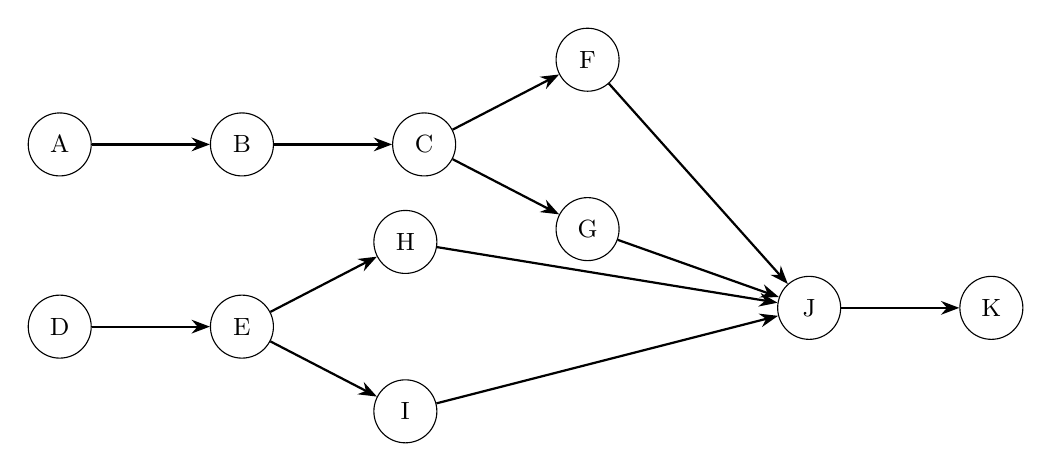
\begin{tikzpicture}[
				node distance=1.2cm and 1.5cm,
				task/.style={circle, draw, minimum size=0.8cm, font=\small},
				arrow/.style={-Stealth, thick}
				]
				% 第一层
				\node[task] (A) {A};
				\node[task, right=of A] (B) {B};
				\node[task, right=of B] (C) {C};
				
				% C的分支
				\node[task, above right=0.5cm and 1.5cm of C] (F) {F};
				\node[task, below right=0.5cm and 1.5cm of C] (G) {G};
				
				% 第二层起始
				\node[task, below=1.5cm of A] (D) {D};
				\node[task, right=of D] (E) {E};
				
				% E的分支
				\node[task, above right=0.5cm and 1.5cm of E] (H) {H};
				\node[task, below right=0.5cm and 1.5cm of E] (I) {I};
				
				% 汇聚点 J
				\node[task, right=2cm of G, yshift=-1cm] (J_real) {J};
				
				% 终点 K
				\node[task, right=of J_real] (K) {K};
				
				% 连线
				\draw[arrow] (A) -- (B);
				\draw[arrow] (B) -- (C);
				\draw[arrow] (C) -- (F);
				\draw[arrow] (C) -- (G);
				
				\draw[arrow] (D) -- (E);
				\draw[arrow] (E) -- (H);
				\draw[arrow] (E) -- (I);
				
				\draw[arrow] (F) -- (J_real);
				\draw[arrow] (G) -- (J_real);
				\draw[arrow] (H) -- (J_real);
				\draw[arrow] (I) -- (J_real);
				
				\draw[arrow] (J_real) -- (K);
				
			\end{tikzpicture}
			\caption{任务依赖关系图}
		\end{figure}
		
		\textbf{任务加工时间表：}
		\begin{center}
			\begin{tabular}{|c|ccccccccccc|}
				\hline
				\textbf{任务} & A & B & C & D & E & F & G & H & I & J & K \\
				\hline
				\textbf{工作站 1 耗时 $t_{i1}$} & 25 & 5 & 5 & 35 & 10 & 7 & 8 & 7 & 2 & 4 & 7 \\
				\textbf{工作站 2 耗时 $t_{i2}$} & 20 & 6 & 4 & 15 & 5 & 5 & 4 & 5 & 10 & 4 & 2 \\
				\hline
			\end{tabular}
		\end{center}
		
		\textbf{问题分析：}
		\begin{itemize}
			\item 问题的关键是确定任务开始加工的次序。
			\item $S_{ij}$ 代表任务 $i$ 在工作站 $j$ 的开始时间，$t_{ij}$ 代表任务 $i$ 在工作站 $j$ 的加工时间。
			\item $P_i$ 表示任务 $i$ 的前置任务的集合（例如 $P_B = \{A\}$，$P_C = \{B\}$，$P_J = \{F, G, H, I\}$）。
		\end{itemize}
		
		\textbf{决策变量：}
		\begin{itemize}
			\item $S_{ij}$ 代表任务 $i$ 在工作站 $j$ 的开始时间，$i = 1, 2, \dots, 11,\ j = 1, 2$。
			\item $q_{1ikj}, q_{2ikj}$：用于处理任务 $i$ 和 $k$ 在同一工作站 $j$ 上的顺序的 0-1 变量。
			\item $q_{1ikj}=1$代表$i$在$k$前，$q_{2ikj}=1$代表$k$在$i$前。
		\end{itemize}
		
		\textbf{目标函数：}
		\begin{itemize}
			\item 最小化最后一个任务 $K$（即任务 11）通过工作站 2 的时间，使总装配时间最短。
			\[
			\min C := S_{11,2} + t_{11,2}
			\]
		\end{itemize}
		
		\textbf{约束条件：}
		\begin{enumerate}
			\item \textbf{任务优先顺序约束}：如果任务 $k$ 是任务 $i$ 的前置任务，则必须满足：
			\[
			S_{k2} + t_{k2} \le S_{i1}, \quad \forall k \in P_i
			\]
			（前置任务 $k$ 在工作站 2 结束才能开始任务 $i$ 在工作站 1 的加工）
			
			\item \textbf{工作站不可以同时进行两个任务的加工}：
			对于同一工作站 $j$，任务 $i$ 和 $k$ 不能同时进行，即 $S_{ij} + t_{ij} \le S_{kj}$ 或 $S_{kj} + t_{kj} \le S_{ij}$。
			\[
			\begin{cases}
				S_{ij} + t_{ij} \le S_{kj} + M(1 - q_{1ikj}), & i, k = 1, \dots, 11; j = 1, 2 \\
				S_{kj} + t_{kj} \le S_{ij} + M(1 - q_{2ikj}), & i, k = 1, \dots, 11; j = 1, 2 \\
				q_{1ikj} + q_{2ikj} \ge 1, & i, k = 1, \dots, 11; j = 1, 2 \\
				q_{1ikj}, q_{2ikj} \in \{0,1\}, & i, k = 1, \dots, 11; j = 1, 2
			\end{cases}
			\]
			其中 $M$ 为一个足够大的数。
			
			\item \textbf{工作站顺序约束}：每个任务 $i$ 必须先经过工作站 1 再经过工作站 2：
			\[
			S_{i1} + t_{i1} \le S_{i2}, \quad i = 1, 2, \dots, 11
			\]
			
			\item \textbf{非负整数约束}：
			\[
			S_{ij} \in \mathbb{Z}_+, \quad i = 1, 2, \dots, 11,\ j = 1, 2
			\]
		\end{enumerate}
		
		\bigskip
		\textbf{该问题对应的 LP 模型为：}
		\[
		\begin{aligned}
			\min \quad & C := S_{11,2} + t_{11,2} \\
			\text{s.t.} \quad & \left\{
			\begin{aligned}
				& S_{k2} + t_{k2} \le S_{i1}, \quad \forall k \in P_i && \text{(任务优先)} \\
				& S_{ij} + t_{ij} \le S_{kj} + M(1 - q_{1ikj}), && i, k = 1, \dots, 11; j = 1, 2 \\
				& S_{kj} + t_{kj} \le S_{ij} + M(1 - q_{2ikj}), && i, k = 1, \dots, 11; j = 1, 2 \\
				& q_{1ikj} + q_{2ikj} \ge 1, && i, k = 1, \dots, 11; j = 1, 2 \\
				& q_{1ikj}, q_{2ikj} \in \{0,1\}, && i, k = 1, \dots, 11; j = 1, 2 \\
				& S_{i1} + t_{i1} \le S_{i2}, && i = 1, 2, \dots, 11 && \text{(工作站顺序)} \\
				& S_{ij} \in \mathbb{Z}_+, && i = 1, 2, \dots, 11,\ j = 1, 2
			\end{aligned}
			\right.
		\end{aligned}
		\]
	\end{example}
	
	\subsubsection{例题 10-3：装配线问题 (任务分配)}
	
	\textbf{问题描述：}
	11 件任务 (A-K) 分配到 4 个工作站 (1-4)，任务间的依赖关系如下图（后续节点任务的启动需要前序任务的完成），每件任务所花费的时间如下表：
	
	% --- 这是一个用 TikZ 还原的依赖关系图 ---
	\begin{figure}[H]
		\centering
		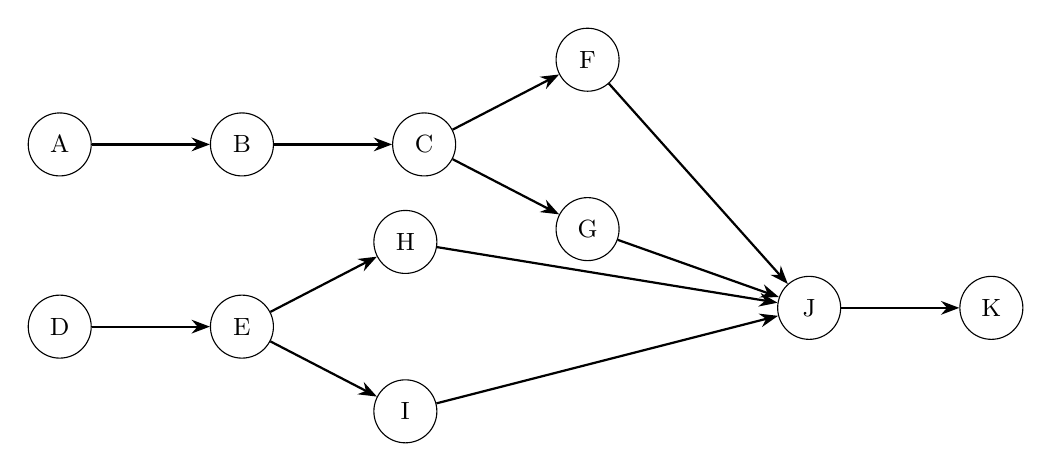
\begin{tikzpicture}[
			node distance=1.2cm and 1.5cm,
			task/.style={circle, draw, minimum size=0.8cm, font=\small},
			arrow/.style={-Stealth, thick}
			]
			% 第一层
			\node[task] (A) {A};
			\node[task, right=of A] (B) {B};
			\node[task, right=of B] (C) {C};
			
			% C的分支
			\node[task, above right=0.5cm and 1.5cm of C] (F) {F};
			\node[task, below right=0.5cm and 1.5cm of C] (G) {G};
			
			% 第二层起始
			\node[task, below=1.5cm of A] (D) {D};
			\node[task, right=of D] (E) {E};
			
			% E的分支
			\node[task, above right=0.5cm and 1.5cm of E] (H) {H};
			\node[task, below right=0.5cm and 1.5cm of E] (I) {I};
			
			% 汇聚点 J
			%\node[task, right=4cm of E] (J) {J}; % 粗略定位
			% 为了让图好看，微调 J 的位置，使其处于 F,G,H,I 的右侧
			\node[task, right=2cm of G, yshift=-1cm] (J_real) {J}; 
			
			% 终点 K
			\node[task, right=of J_real] (K) {K};
			
			% 连线
			\draw[arrow] (A) -- (B);
			\draw[arrow] (B) -- (C);
			\draw[arrow] (C) -- (F);
			\draw[arrow] (C) -- (G);
			
			\draw[arrow] (D) -- (E);
			\draw[arrow] (E) -- (H);
			\draw[arrow] (E) -- (I);
			
			\draw[arrow] (F) -- (J_real);
			\draw[arrow] (G) -- (J_real);
			\draw[arrow] (H) -- (J_real);
			\draw[arrow] (I) -- (J_real);
			
			\draw[arrow] (J_real) -- (K);
			
		\end{tikzpicture}
		\caption{任务依赖关系图}
	\end{figure}
	
	\begin{table}[H]
		\centering
		\small
		\begin{tabular}{c|ccccccccccc}
			\toprule
			\textbf{任务 ($i$)} & A & B & C & D & E & F & G & H & I & J & K \\
			\midrule
			\textbf{时间 ($t_i$)} & 45 & 11 & 9 & 50 & 15 & 12 & 12 & 12 & 12 & 8 & 9 \\
			\bottomrule
		\end{tabular}
		\caption{各任务所需时间表}
	\end{table}
	
	\noindent 设计装配任务分配方案，目标是为每个工作站分配加工任务，尽可能使总装配时间最短。
	
	\begin{solution}
		\textbf{问题分析：}
		\begin{itemize}
			\item $t_i$ 为任务 $i$ 的执行时间，$P_i$ 是任务 $i$ 前置任务的集合。
		\end{itemize}
		
		\textbf{决策变量：}
		\begin{enumerate}
			\item \textbf{任务分配变量}：任务 $i$ 是否分配到工作站 $j$：
			\[
			x_{ij} = \begin{cases}
				1, & \text{如果任务 } i \text{ 被分配到工作站 } j \\
				0, & \text{否则}
			\end{cases}
			\]
			其中 $i = 1, 2, \dots, 11;\ j = 1, 2, 3, 4$。
			
			\item \textbf{时间变量}：任务 $i$ 的开始时间 $S_i$。
		\end{enumerate}
		
		\textbf{目标函数：}
		\begin{itemize}
			\item 最小化最后一个任务（或整体完工时间） $T$，即：
			\[
			\min T
			\]
			（注：需满足 $T \ge S_i + t_i$）
		\end{itemize}
		
		\textbf{约束条件：}
		\begin{enumerate}
			\item \textbf{唯一性约束}：每个任务必须分配到唯一一个工作站：
			\[
			\sum_{j=1}^{4} x_{ij} = 1, \quad i = 1, 2, \dots, 11
			\]
			
			\item \textbf{前置任务约束}：任务 $i$ 的开始时间受其前置任务 $k$ 的约束：
			\[
			S_i \ge S_k + t_k, \quad \forall k \in P_i
			\]
			
			\item \textbf{同一工作站任务不重叠约束}（引入辅助变量）：
			为了避免同一工作站上的任务时间冲突，引入 0-1 变量 $v_{ikj}$ 表示任务 $i$ 和 $k$ 是否同时分配在工作站 $j$，以及 $q_{1ik}, q_{2ik}$ 用于确定先后顺序。
			
			若 $x_{ij}=x_{kj}=1$，则必须满足 $S_i \ge S_k + t_k$ 或 $S_k \ge S_i + t_i$。转化为线性约束如下：
			\[
			\begin{cases}
				v_{ikj} \le x_{ij} \\
				v_{ikj} \le x_{kj} \\
				v_{ikj} \ge x_{ij} + x_{kj} - 1 \qquad \text{这三行说明} v_{ikj}=x_{ij}\times x_{kj}\\
				S_i \ge S_k + t_k - M(1 - q_{1ik}) \\
				S_k \ge S_i + t_i - M(1 - q_{2ik}) \\
				q_{1ik} + q_{2ik} < 2 \\
				q_{1ik} + q_{2ik} \ge \sum_{j=1}^{4} v_{ikj}
			\end{cases}
			\]
		\end{enumerate}
		
		\bigskip
		\textbf{该问题对应的 LP 模型为：}
		\[
		\begin{aligned}
			\min \quad & T \\
			\text{s.t.} \quad & \left\{
			\begin{aligned}
				& \sum_{j=1}^{4} x_{ij} = 1, \quad i = 1, 2, \dots, 11 \\
				& S_i \ge S_k + t_k, \quad \forall k \in P_i \\
				& v_{ikj} \le x_{ij}, \quad i, k = 1, \dots, 11, j = 1, \dots, 4 \\
				& v_{ikj} \le x_{kj}, \quad i, k = 1, \dots, 11, j = 1, \dots, 4 \\
				& v_{ikj} \ge x_{ij} + x_{kj} - 1, \quad i, k = 1, \dots, 11, j = 1, \dots, 4 \\
				& S_i \ge S_k + t_k - M(1 - q_{1ik}), \quad i, k = 1, \dots, 11 \\
				& S_k \ge S_i + t_i - M(1 - q_{2ik}), \quad i, k = 1, \dots, 11 \\
				& q_{1ik} + q_{2ik} \ge \sum_{j=1}^{4} v_{ikj}, \quad i, k = 1, \dots, 11 \\
				& q_{1ik} + q_{2ik} < 2, \quad i, k = 1, \dots, 11 \\
				& T \ge S_i + t_i, \quad i = 1, 2, \dots, 11 \\
				& q_{1ik}, q_{2ik}, v_{ikj}, x_{ij} \in \{0, 1\}
			\end{aligned}
			\right.
		\end{aligned}
		\]
	\end{solution}
	
	\section{非线性规划}
	
	本节讨论无约束问题：
	\begin{equation}
		\min_{x \in \mathbb{R}^n} f(x) \tag{3.1}
	\end{equation}
	
	\subsection{无约束问题的最优性条件}
	
	\begin{theorem}[一阶必要条件]
		设 $x^*$ 是 (3.1) 的一个局部极小点，且 $f(x)$ 在 $x^*$ 的邻域上连续可微，则 $f'(x^*) = 0$，即：
		\begin{equation}
			\nabla f(x^*) = f'(x^*) = \left( \frac{\partial f(x^*)}{\partial x_1}, \dots, \frac{\partial f(x^*)}{\partial x_n} \right)^T = 0
		\end{equation}
		称满足上式的点为\textbf{驻点}（稳定点）。实际上，在区域内部，极值点必为驻点，但驻点却不一定是极值点。
	\end{theorem}
	
	\begin{theorem}[二阶必要条件]
		设 $x^*$ 是 (3.1) 的一个局部极小点，且 $f(x)$ 在 $x^*$ 的邻域上二阶连续可微，则：
		\begin{enumerate}
			\item $\nabla f(x^*) = 0$;
			\item $\nabla^2 f(x^*)$ 为半正定矩阵（Positive Semidefinite）。
		\end{enumerate}
	\end{theorem}
	
	\begin{theorem}[极值存在的二阶充分条件]
		设 $f(x)$ 在 $x^*$ 的邻域上二阶连续可微，且 $\nabla f(x^*) = 0$，若 Hessian 矩阵 $\nabla^2 f(x^*)$ 是\textbf{正定矩阵}（Positive Definite），则 $x^*$ 为 (3.1) 的一个局部极小点。
	\end{theorem}
	
	\begin{theorem}[凸函数取得极值的充要条件]
		设 $f(x)$ 是一阶连续可微的凸函数，则 $x^*$ 是 $\min f(x)$ 的全局极小点的充要条件是 $\nabla f(x^*) = 0$。
		\begin{quote}
			注：一般来说，目标函数的稳定点不一定是极小点，但对于目标函数是凸函数的无约束优化问题：
			\[ \text{稳定点} = \text{局部极小点} = \text{全局极小点} \]
		\end{quote}
	\end{theorem}
	
	\subsection{等式约束优化与拉格朗日乘子法}
	
	对于包含等式约束的非线性规划问题：
	\begin{equation}
		\begin{aligned}
			\min \quad & f(x) \\
			\text{s.t.} \quad & h_k(x) = 0, \quad k=1,\dots,l
		\end{aligned}
	\end{equation}
	
	我们使用\textbf{拉格朗日乘子法}（Lagrange Multiplier Method）求解。
	
	\subsubsection*{求解方法}
	1. \textbf{构造拉格朗日函数}：引入乘子 $\lambda = (\lambda_1, \dots, \lambda_l)^T$，构造函数：
	\[ L(x, \lambda) = f(x) + \sum_{k=1}^{l} \lambda_k h_k(x) \]
	2. \textbf{建立方程组}：对 $x$ 和 $\lambda$ 求偏导并令其为 0：
	\[
	\begin{cases}
		\nabla_x L(x, \lambda) = \nabla f(x) + \sum_{k=1}^{l} \lambda_k \nabla h_k(x) = 0 \\
		\nabla_\lambda L(x, \lambda) = h(x) = 0
	\end{cases}
	\]
	3. \textbf{求解}：解上述方程组得到的点 $(x^*, \lambda^*)$ 即为可能的极值点。
	
	\begin{example}[非线性规划求解]
		求解下列非线性规划问题：
		\[
		\begin{aligned}
			\min \quad & f(X) = x_1^2 - x_1 x_2 + x_2^2 - 10x_1 - 4x_2 + 60 \\
			\text{s.t.} \quad & h(X) = x_1 + x_2 - 8 = 0
		\end{aligned}
		\]
	\end{example}
	
	\begin{solution}
		构造拉格朗日函数：
		\[ L(x, \lambda) = x_1^2 - x_1 x_2 + x_2^2 - 10x_1 - 4x_2 + 60 + \lambda(x_1 + x_2 - 8) \]
		由一阶必要条件：
		\[
		\begin{cases}
			\frac{\partial L}{\partial x_1} = 2x_1 - x_2 + \lambda - 10 = 0 \\
			\frac{\partial L}{\partial x_2} = -x_1 + 2x_2 + \lambda - 4 = 0 \\
			\frac{\partial L}{\partial \lambda} = x_1 + x_2 - 8 = 0
		\end{cases}
		\]
		解得 $X_1^* = 5, X_2^* = 3, \lambda^* = 3$。
		
		检查 $f(X)$ 的 Hessian 矩阵：
		\[ H(X) = \begin{pmatrix} 2 & -1 \\ -1 & 2 \end{pmatrix} \]
		一阶主子式 $2 > 0$，二阶主子式 $4-1=3 > 0$，故矩阵正定。
		因此 $f(X)$ 为严格凸函数，所以 $X^*=(5,3)$ 为全局最优解，最小值为 $f(X^*) = 17$。
	\end{solution}
	
	\subsection{不等式约束优化与 KT 条件}
	
	对于包含不等式约束的问题：
	\begin{equation}
		\begin{aligned}
			\min \quad & f(x) \\
			\text{s.t.} \quad & g_i(x) \le 0, \quad i=1,\dots,m 
		\end{aligned}
		\tag{3.3}  % <--- 移到这里来
	\end{equation}
	
	\begin{theorem}[KT 条件 / KKT 条件]
		设 $x^*$ 是不等式约束问题 (3.3) 的局部极小点，有效约束集 $I(x^*) = \{i \mid g_i(x^*) = 0\}$。若向量组 $\nabla g_i(x^*) (i \in I(x^*))$ 线性无关，则存在向量 $\lambda^* = (\lambda_1^*, \dots, \lambda_m^*)^T$，使得：
		\begin{equation}
			\begin{cases}
				\nabla f(x^*) + \sum_{i=1}^{m} \lambda_i^* \nabla g_i(x^*) = 0 & \text{(平稳性条件)} \\
				g_i(x^*) \le 0 & \text{(原问题可行性)} \\
				\lambda_i^* \ge 0 & \text{(对偶可行性)} \\
				\lambda_i^* g_i(x^*) = 0, \quad (i=1,\dots,m) & \text{(互补松弛条件)}
			\end{cases}
		\end{equation}
		满足 KT 条件的点称为 \textbf{KT 点}。
	\end{theorem}
	
	\subsubsection*{补充：如何利用 KT 条件进行计算 (CS 方法)}
	KT 条件的核心难点在于处理\textbf{互补松弛条件} $\lambda_i g_i(x) = 0$。这意味着对于每一个约束 $i$，要么乘子 $\lambda_i = 0$，要么约束取等号 $g_i(x) = 0$（即约束起作用）。
	
	\textbf{手工计算步骤（分类讨论法）：}
	\begin{enumerate}
		\item \textbf{构造拉格朗日函数}：$L(x, \lambda) = f(x) + \sum \lambda_i g_i(x)$。
		\item \textbf{列出方程组}：写出上述定理中的 4 个 KT 条件。
		\item \textbf{情形分类}：假设有 $m$ 个不等式约束，需要讨论 $2^m$ 种情况。
		\begin{itemize}
			\item \textbf{情形 1（约束无效）}：假设 $\lambda_i = 0$。此时代入 $\nabla_x L = 0$ 求解 $x$，然后验证是否满足 $g_i(x) \le 0$。
			\item \textbf{情形 2（约束有效）}：假设 $g_i(x) = 0$（即边界上）。此时利用方程组求解 $x$ 和 $\lambda_i$，然后验证是否满足 $\lambda_i \ge 0$。
		\end{itemize}
		\item \textbf{比较选优}：找出所有满足条件的候选点（KT点），比较目标函数值确定最优解。
	\end{enumerate}
	
	
	\begin{example}
		某企业的生产函数 $Q = 3K^{1/3}L^{1/2}$，它表示在资本投入 $K$ 和劳动投入 $L$ 时，某种产品的产出量为 $Q$。若产品价格为 $P=4$，要素投入价格分别为 $P_K=4, P_L=3$，试求该企业得到最大利润时要素投入水平。
	\end{example}
	
	\begin{solution}
		该企业的利润函数为：
		\[ 
		\begin{aligned}
			Y &= P \cdot Q - P_K \cdot K - P_L \cdot L \\
			&= 12K^{1/3}L^{1/2} - 4K - 3L
		\end{aligned}
		\]
		这是一个无约束极大值问题：$\max Y = 12K^{1/3}L^{1/2} - 4K - 3L$。
		
		求解一阶导数并令其为 0：
		\[
		\begin{cases}
			\frac{\partial Y}{\partial K} = 12 \cdot \frac{1}{3} K^{-2/3} L^{1/2} - 4 = 4K^{-2/3}L^{1/2} - 4 = 0 \\
			\frac{\partial Y}{\partial L} = 12 \cdot \frac{1}{2} K^{1/3} L^{-1/2} - 3 = 6K^{1/3}L^{-1/2} - 3 = 0
		\end{cases}
		\]
		化简方程组：
		\begin{itemize}
			\item 由第一式得：$K^{-2/3}L^{1/2} = 1 \Rightarrow L^{1/2} = K^{2/3} \Rightarrow L = K^{4/3}$
			\item 代入第二式：$2K^{1/3}(K^{4/3})^{-1/2} = 1 \Rightarrow 2K^{1/3}K^{-2/3} = 1 \Rightarrow 2K^{-1/3} = 1$
		\end{itemize}
		解得：$K = 8$，代回得 $L = 8^{4/3} = 16$。
		
		\textbf{检验二阶条件}：
		在驻点处的 Hessian 矩阵为：
		\[
		H(K, L) = \begin{pmatrix} 
			\frac{\partial^2 Y}{\partial K^2} & \frac{\partial^2 Y}{\partial K \partial L} \\
			\frac{\partial^2 Y}{\partial L \partial K} & \frac{\partial^2 Y}{\partial L^2}
		\end{pmatrix}
		= \begin{pmatrix}
			-\frac{1}{3} & \frac{1}{8} \\
			\frac{1}{8} & -\frac{3}{32}
		\end{pmatrix}
		\]
		（注：此处数值由代入 $K=8, L=16$ 计算得出）。
		
		\begin{itemize}
			\item 一阶主子式：$D_1 = -1/3 < 0$
			\item 二阶主子式：$D_2 = (-1/3)(-3/32) - (1/8)^2 = 3/96 - 1/64 > 0$
		\end{itemize}
		故 $H$ 为负定矩阵，函数在 $(8, 16)$ 处取得极大值。
		
		\textbf{结论}：当投入 $K=8, L=16$ 时，企业可获得最大利润 $Y_{\max}=16$，此时产量为 $Q = 3 \times 8^{1/3} \times 16^{1/2} = 24$。
	\end{solution}
	
	\begin{example}[利用 KKT 条件求解不等式约束]
		求解如下非线性规划问题：
		\[
		\begin{aligned}
			\min \quad & f(x) = (x_1 - 2)^2 + x_2^2 \\
			\text{s.t.} \quad & x_1 + x_2 \le 1
		\end{aligned}
		\]
	\end{example}
	
	\begin{solution}
		\textbf{第一步：形式转化与构造函数} \\
		将约束条件写为标准形式 $g(x) = x_1 + x_2 - 1 \le 0$。
		构造拉格朗日函数：
		\[ L(x, \lambda) = (x_1 - 2)^2 + x_2^2 + \lambda(x_1 + x_2 - 1) \]
		
		\textbf{第二步：列出 KKT 条件} \\
		根据定理，最优解必须满足以下条件组：
		\[
		\begin{cases}
			\nabla_x L = 0 \Rightarrow 
			\begin{cases} 
				2(x_1 - 2) + \lambda = 0 & \text{\textcircled{1}} \\
				2x_2 + \lambda = 0       & \text{\textcircled{2}}
			\end{cases} \\
			\lambda (x_1 + x_2 - 1) = 0  \quad \text{(互补松弛条件) \textcircled{3}} \\
			x_1 + x_2 - 1 \le 0, \quad \lambda \ge 0 \quad \text{(可行性条件)}
		\end{cases}
		\]
		
		\textbf{第三步：分类讨论求解} \\
		根据互补松弛条件 \textcircled{3}，分两种情况讨论：
		
		\begin{itemize}
			\item \textbf{情形 1：} 假设 $\lambda = 0$（即约束不起作用）。
			代入方程 \textcircled{1} 和 \textcircled{2}，解得：
			\[ x_1 = 2, \quad x_2 = 0 \]
			检验可行性：$x_1 + x_2 = 2 + 0 = 2 > 1$，违反约束条件，故此解无效。
			
			\item \textbf{情形 2：} 假设 $\lambda > 0$（即约束起作用，点在边界上）。
			由 \textcircled{3} 可知 $x_1 + x_2 - 1 = 0 \Rightarrow x_1 + x_2 = 1$。
			由 \textcircled{1} 和 \textcircled{2} 消去 $\lambda$：
			\[ 2(x_1 - 2) = 2x_2 \implies x_1 - x_2 = 2 \]
			联立方程组：
			\[
			\begin{cases}
				x_1 + x_2 = 1 \\
				x_1 - x_2 = 2
			\end{cases}
			\]
			解得 $x_1 = 1.5, \quad x_2 = -0.5$。
			此时由 \textcircled{2} 求得 $\lambda = -2(-0.5) = 1$，满足 $\lambda \ge 0$。
		\end{itemize}
		
		\textbf{结论：} \\
		该问题的全局最优解为 $x^* = (1.5, -0.5)$，最小值为：
		\[ f_{\min} = (1.5 - 2)^2 + (-0.5)^2 = 0.25 + 0.25 = 0.5 \]
	\end{solution}
	
	\section{动态规划}
	
	\subsection{有限期确定动态规划 (核心考点整理)}
	
	动态规划 (Dynamic Programming, DP) 的核心在于最优性原理：一个最优策略的子策略总是最优的。在考试中，最关键的是定义状态和写出状态转移方程（递推公式）。
	
	\subsubsection{解题通用步骤}
	\begin{enumerate}
		\item \textbf{划分阶段} ($k$)：将过程划分为若干相互联系的阶段。
		\item \textbf{确定状态} ($s_k$)：描述每个阶段开始时的客观条件（无后效性）。
		\item \textbf{确定决策} ($x_k$)：从当前状态转移到下一状态的选择。
		\item \textbf{写出方程}：建立指标函数 $f_k(s_k)$ 的递推关系（核心）。
		\item \textbf{边界条件}：确定初始或结束条件的数值。
	\end{enumerate}
	
	\subsubsection{五大经典模型与例题解析}
	
	\paragraph{1. 最短路问题 (Shortest Path)}
	\textbf{模型}：在分层图中，求起点 $A$ 到终点 $G$ 的最短路径。
	\begin{itemize}
		\item \textbf{递推方程 (逆序法)}：
		设 $f_k(u)$ 为从当前节点 $u$ 到终点 $G$ 的最短距离：
		\[
		f_k(u) = \min_{v \in N^+(u)} \{ d(u,v) + f_{k+1}(v) \}
		\]
		其中 $d(u,v)$ 是边长，$N^+(u)$ 是 $u$ 的后继节点集合。
		\item \textbf{边界条件}：$f_{EndPoint}(G) = 0$。
		\item \textbf{计算技巧}：使用\textbf{标号法}，从终点向起点逆推，在图上直接标记每个节点到终点的最短距离。
	\end{itemize}
	
	\paragraph{2. 资源分配/投资问题 (Resource Allocation)}
	\textbf{模型}：将总资源 $a$ 分配给 $n$ 个工程/部门，第 $i$ 个工程分 $x_i$ 获利 $g_i(x_i)$，求总利润最大。
	\begin{itemize}
		\item \textbf{定义}：$f_k(x)$ 表示将资源 $x$ 分配给\textbf{前 $k$ 个}工厂所得的最大利润。
		\item \textbf{递推方程 (顺序法)}：
		\[
		f_k(x) = \max_{0 \le y \le x} \{ g_k(y) + f_{k-1}(x-y) \}
		\]
		其中 $y$ 为分给第 $k$ 个工厂的资源，$x-y$ 为留给前 $k-1$ 个工厂的资源。
		\item \textbf{解题表格法}：
		考试通常给出离散数据表，需画表计算。
		\begin{itemize}
			\item 第1阶段：$f_1(x) = g_1(x)$。
			\item 第2至 $n$ 阶段：列表枚举所有可能的 $y$，计算 $g_k(y) + f_{k-1}(x-y)$ 找最大值。
		\end{itemize}
	\end{itemize}
	
	\paragraph{3. 0-1 背包问题 (Knapsack Problem)}
	\textbf{模型}：$n$ 种物品，重量 $a_j$，价值 $c_j$，背包容量 $b$。每种物品选或不选 ($x_j \in \{0,1\}$)。
	\begin{itemize}
		\item \textbf{定义}：$z_k(d)$ 表示在前 $k$ 个物品中选择，总重量不超过 $d$ 的最大价值。
		\item \textbf{递推方程}：
		\[
		z_k(d) = 
		\begin{cases} 
			z_{k-1}(d), & \text{若 } a_k > d \text{ (装不下)} \\
			\max \{ z_{k-1}(d), \ c_k + z_{k-1}(d - a_k) \}, & \text{若 } a_k \le d \text{ (能装下，选或不选)}
		\end{cases}
		\]
		\item \textbf{复杂度}：运算次数为 $O(nb)$。
	\end{itemize}
	
	\paragraph{4. 旅行商问题 (TSP)}
	\textbf{模型}：从城市0出发，经过所有城市一次且仅一次，最后回到0，求最短路径。
	\begin{itemize}
		\item \textbf{状态定义}：$(i, S)$，表示当前在城市 $i$，\textbf{还需要}经过集合 $S$ 中的城市回到0。
		\item \textbf{递推方程}：
		\[
		g_k(i, S) = \min_{j \in S} \{ d_{ij} + g_{k-1}(j, S \setminus \{j\}) \}
		\]
		\item \textbf{边界条件}：$g_0(i, \emptyset) = d_{i0}$ (从 $i$ 直接回起点)。
		\item \textbf{注意}：随着阶段 $k$ 增加，$S$ 的规模减小，计算量指数级增长。
	\end{itemize}
	
	\paragraph{5. 连续变量问题 (几何规划等)}
	\textbf{模型}：决策变量 $x_k$ 是连续的，通常涉及乘积最大化或非线性函数。
	\begin{itemize}
		\item \textbf{例题}：$\max z = x_1^2 x_2 x_3^3$，s.t. $\sum x_i \le 6, x_i \ge 0$。
		\item \textbf{解法}：利用微分法求极值。
		\item \textbf{步骤}：
		\begin{enumerate}
			\item 写出方程：$f_k(s_k) = \max_{0 \le x_k \le s_k} \{ r_k(x_k) \cdot f_{k+1}(s_k - x_k) \}$。
			\item 逆向求解：先求 $f_3$，再求 $f_2$ (对 $x_2$ 求导令为0找到最优 $x_2$ 与 $s_2$ 的关系)，最后求 $f_1$。
		\end{enumerate}
	\end{itemize}
	
	\subsubsection{凸函数性质简化 (针对资源分配)}
	若收益函数 $g(x), h(x)$ 均为凸函数且 $g(0)=h(0)=0$，则最优决策一定在端点处取得（即全部投入A或全部投入B），无需遍历中间值。
	\[
	f_k(x) = \max \{ h(x) + f_{k-1}(bx), \ g(x) + f_{k-1}(ax) \}
	\]
	此定理可将计算量从枚举简化为比较两个端点值。
	
	\subsection{不定期多阶段决策问题 (一般图最短路)}
	
	与有限期问题不同，一般图上的最短路问题（如路由选择、网络流）可能包含回路，且阶段数 $k$ 不固定（不确定需要走几步）。这类问题的核心在于求解函数方程。
	
	\subsubsection{核心模型与方程}
	\textbf{问题描述}：在加权有向/无向图 $G=(V,E)$ 中，求各节点 $i$ 到汇点（终点）$v_n$ 的最短距离。
	
	\textbf{贝尔曼函数方程 (Bellman Equation)}：
	设 $f(i)$ 为节点 $i$ 到终点 $v_n$ 的最短距离，则满足：
	\begin{equation}
		\begin{cases} 
			f(i) = \min_{j \in V} \{ c_{ij} + f(j) \}, & i \neq n \\
			f(n) = 0 
		\end{cases}
	\end{equation}
	其中 $c_{ij}$ 为边 $(i,j)$ 的权值。此方程通常有两种迭代解法。
	
	\subsubsection{解法一：函数空间迭代法 (Value Iteration)}
	此方法等价于限制了“最大允许步数”的递推。
	\begin{enumerate}
		\item \textbf{定义}：$f_k(i)$ 表示从 $i$ 到终点，经过边数 $\le k$ 条的最短路长度。
		\item \textbf{迭代公式}：
		\[
		f_k(i) = \min_{j} \{ c_{ij} + f_{k-1}(j) \}
		\]
		\item \textbf{边界条件}：$f_0(n)=0$，其余 $f_0(i)=\infty$（或根据 $k=1$ 直接初始化为直达距离）。
		\item \textbf{收敛性}：序列 $\{f_k(i)\}$ 单调下降收敛于最优解 $f(i)$。当 $f_k(i) = f_{k-1}(i)$ 时迭代结束。
	\end{enumerate}
	
	\subsubsection{解法二：策略空间迭代法 (Policy Iteration)}
	此方法通过不断改进“行走策略”来逼近最优解，通常比函数空间迭代收敛更快。
	
	\begin{enumerate}
		\item \textbf{定义策略 $s(i)$}：对于每个节点 $i$，指定其下一个去往的节点（后继）为 $s(i)$。
		\item \textbf{算法步骤}：
		\begin{itemize}
			\item \textbf{Step 0 初始化}：选取任意初始策略 $s_0$（例如直达终点）。
			\item \textbf{Step 1 策略评估 (Policy Evaluation)}：
			求解在当前策略 $s_k$ 下的距离 $f_k$。即解线性方程组：
			\[
			f_k(i) = c_{i, s_k(i)} + f_k(s_k(i)), \quad (i=1 \dots n-1)
			\]
			\item \textbf{Step 2 策略改进 (Policy Update)}：
			利用 $f_k$ 寻找更优的后继节点，更新策略：
			\[
			s_{k+1}(i) = \arg\min_{j} \{ c_{ij} + f_k(j) \}
			\]
			\item \textbf{Step 3 终止判定}：若 $s_{k+1}(i)$ 与 $s_k(i)$ 完全相同，则停止，当前 $f_k$ 即为最短路。
		\end{itemize}
	\end{enumerate}
	
	\subsubsection{经典例题解析}
	\textbf{题目}：已知图的节点 $v_1 \dots v_5$（$v_5$为终点），各边权值如下，求 $v_1$ 到 $v_5$ 的最短路。
	\begin{itemize}
		\item $v_1$ 连边：$v_5(7), v_2(6), v_3(2), v_4(5)$
		\item $v_2$ 连边：$v_5(2), v_3(0.5), v_4(5)$
		\item $v_3$ 连边：$v_5(5), v_4(1)$
		\item $v_4$ 连边：$v_5(3)$
	\end{itemize}
	
	\textbf{解法演示 (使用策略空间迭代法)}：
	
	\textbf{1. 初始策略 $s_0$}：
	假设所有点都直达 $v_5$（若无直达边则设为无穷大，此处均有）。
	\[ s_0 = \{ v_1 \to v_5, v_2 \to v_5, v_3 \to v_5, v_4 \to v_5 \} \]
	\textbf{求解 $f_0$} (直接代入权值)：
	\[ f_0(1)=7, \ f_0(2)=2, \ f_0(3)=5, \ f_0(4)=3, \ f_0(5)=0 \]
	
	\textbf{2. 第一次迭代 (改进策略)}：
	计算 $c_{ij} + f_0(j)$ 寻找最小值的索引 $j$。
	\begin{itemize}
		\item $v_1$: $\min \{ 7+0(v_5), 6+2(v_2), 2+5(v_3), 5+3(v_4) \} = 7 \to$ 保持 $v_5$
		\item $v_2$: $\min \{ 2+0(v_5), 0.5+5(v_3), 5+3(v_4) \} = 2 \to$ 保持 $v_5$ （注：$0.5+5=5.5 > 2$）
		\item $v_3$: $\min \{ 5+0(v_5), 1+3(v_4) \} = 4 \to$ \textbf{改为去 $v_4$} (因为 $4 < 5$)
		\item $v_4$: $\min \{ 3+0(v_5), \dots \} = 3 \to$ 保持 $v_5$
	\end{itemize}
	新策略 $s_1$: $v_3 \to v_4$，其余直达 $v_5$。
	
	\textbf{3. 第二次迭代 (评估与更新)}：
	\textbf{评估 $s_1$} (解方程)：
	\[
	\begin{cases}
		f_1(4) = 3 + 0 = 3 \\
		f_1(3) = c_{34} + f_1(4) = 1 + 3 = 4 \\
		f_1(2) = 2 \\
		f_1(1) = 7
	\end{cases}
	\]
	\textbf{更新 $s_2$}：
	再次检查 $v_1$：$\min \{ 7(v_5), 6+2(v_2), \mathbf{2+4(v_3)}, 5+3(v_4) \} = 6$。
	这里 $2+4=6 < 7$，故 $v_1$ 的策略改为去 $v_3$。
	同理检查 $v_2$：$\min \{ 2(v_5), \mathbf{0.5+4(v_3)} \} = 4.5 > 2$，保持不变。
	
	最终策略收敛，最短路径为：$v_1 \to v_3 \to v_4 \to v_5$，长度 $2+1+3=6$（注：原题示例最终收敛值与具体边权有关，此例展示方法流程）。
	
	\subsection{马氏决策规划 (Markov Decision Processes)}
	
	马氏决策规划主要研究在随机环境中，如何通过序贯决策使系统获得最大的期望报酬。其核心在于系统的状态转移具有“无后效性”（马尔可夫性）。
	
	\subsubsection{基本概念与模型要素}
	\begin{enumerate}
		\item \textbf{马尔可夫性 (Markov Property)}：
		系统的未来状态仅与当前状态有关，与过去的历史状态无关。即：
		\[ p(s_{t+1}|s_t, a_t, \dots, s_0) = p(s_{t+1}|s_t, a_t) \]
		\item \textbf{核心四要素}：
		\begin{itemize}
			\item \textbf{状态集合 ($S$)}：环境的所有可能状态。
			\item \textbf{动作/决策集合 ($A$)}：智能体可采取的动作。
			\item \textbf{转移概率 ($P$)}：$p(s'|s,a)$，即在状态 $s$ 采取动作 $a$ 后转移到 $s'$ 的概率。
			\item \textbf{即时奖励 ($R$)}：$r(s, a, s')$，状态转移过程中获得的反馈/收益。
		\end{itemize}
		\item \textbf{一步转移矩阵与报酬矩阵}：
		\begin{itemize}
			\item 转移矩阵 $P = [p_{ij}]$：满足 $\sum_{j} p_{ij} = 1, p_{ij} \ge 0$。
			\item 报酬矩阵 $R = [r_{ij}]$：从状态 $i$ 转移到 $j$ 的收益。
		\end{itemize}
	\end{enumerate}
	
	\subsubsection{核心计算公式}
	
	\paragraph{1. 一步转移期望报酬 $q(i)$}
	表示在状态 $i$ 做出一次转移所能获得的平均收益：
	\[
	q(i) = \sum_{j=1}^{N} p_{ij} r_{ij}
	\]
	若有决策 $d$，则记为 $q^d(i) = \sum_{j} p_{ij}^d r_{ij}^d$。
	
	\paragraph{2. 有限阶段的值迭代方程 (核心考点)}
	设 $f_n(i)$ 为系统处于状态 $i$，距离结束还有 $n$ 个阶段时，采取最优策略能获得的最大总期望报酬。
	
	\textbf{递推公式 (Bellman Optimality Equation)}：
	\[
	f_n(i) = \max_{d \in D} \left\{ q^d(i) + \sum_{j=1}^{N} p_{ij}^d f_{n-1}(j) \right\}, \quad n = 2, 3, \dots
	\]
	\textbf{边界条件 (最后1个阶段)}：
	\[
	f_1(i) = \max_{d \in D} \{ q^d(i) \}
	\]
	
	\subsubsection{经典例题解析：工厂广告决策}
	
	\textbf{题目}：某工厂每月初检查产品销路，状态分为“销路好 (1)”和“销路差 (2)”。
	可选决策：不登广告 (决策1)、登广告 (决策2)。
	求在未来 $n$ 个月内如何决策才能使总期望报酬最大。
	
	\textbf{已知数据}：
	\begin{itemize}
		\item \textbf{决策1 (不登广告)}：
		\[ P^1 = \begin{bmatrix} 0.5 & 0.5 \\ 0.4 & 0.6 \end{bmatrix}, \quad R^1 = \begin{bmatrix} 9 & 3 \\ 3 & -7 \end{bmatrix} \]
		\item \textbf{决策2 (登广告)}：
		\[ P^2 = \begin{bmatrix} 0.8 & 0.2 \\ 0.7 & 0.3 \end{bmatrix}, \quad R^2 = \begin{bmatrix} 4 & 4 \\ 1 & -19 \end{bmatrix} \]
	\end{itemize}
	
	\textbf{解题步骤 (值迭代法)}：
	
	\textbf{Step 1: 计算一步期望报酬向量 $Q$}
	利用公式 $q(i) = \sum p_{ij} r_{ij}$ 计算：
	\begin{itemize}
		\item 决策1：
		$q^1(1) = 0.5 \times 9 + 0.5 \times 3 = 6$
		$q^1(2) = 0.4 \times 3 + 0.6 \times (-7) = 1.2 - 4.2 = -3$
		\item 决策2：
		$q^2(1) = 0.8 \times 4 + 0.2 \times 4 = 4$
		$q^2(2) = 0.7 \times 1 + 0.3 \times (-19) = 0.7 - 5.7 = -5$
	\end{itemize}
	
	\textbf{Step 2: 计算 $n=1$ (只剩1个月) 的最优解}
	\[ f_1(i) = \max \{ q^1(i), q^2(i) \} \]
	\begin{itemize}
		\item 状态1：$\max\{6, 4\} = 6$，最优决策 $d_1(1) = 1$ (不登广告)。
		\item 状态2：$\max\{-3, -5\} = -3$，最优决策 $d_1(2) = 1$ (不登广告)。
		\item 结论：若只剩1个月，无论当前状态如何，都不登广告。
	\end{itemize}
	
	\textbf{Step 3: 计算 $n=2$ (还有2个月) 的最优解}
	公式：$f_2(i) = \max_d \{ q^d(i) + \sum p_{ij}^d f_1(j) \}$。
	已知 $f_1(1)=6, f_1(2)=-3$。
	
	\begin{itemize}
		\item \textbf{对于状态1 (销路好)}：
		\begin{itemize}
			\item 选决策1：$6 + [0.5 \times 6 + 0.5 \times (-3)] = 6 + 1.5 = 7.5$
			\item 选决策2：$4 + [0.8 \times 6 + 0.2 \times (-3)] = 4 + [4.8 - 0.6] = 8.2$
		\end{itemize}
		$\max\{7.5, 8.2\} = 8.2$，故 $f_2(1)=8.2$，最优决策 $d_2(1)=2$ (登广告)。
		
		\item \textbf{对于状态2 (销路差)}：
		\begin{itemize}
			\item 选决策1：$-3 + [0.4 \times 6 + 0.6 \times (-3)] = -3 + [2.4 - 1.8] = -2.4$
			\item 选决策2：$-5 + [0.7 \times 6 + 0.3 \times (-3)] = -5 + [4.2 - 0.9] = -1.7$
		\end{itemize}
		$\max\{-2.4, -1.7\} = -1.7$，故 $f_2(2)=-1.7$，最优决策 $d_2(2)=2$ (登广告)。
	\end{itemize}
	
	\textbf{总结}：
	若规划期为2个月，第一个月的策略是\textbf{无论状态如何都登广告}（因为这能为第二个月创造更好的概率分布），第二个月的策略是不登广告（收割短期利益）。
	
	\subsubsection{详细讲解}
	\begin{itemize}
		\item \textbf{状态空间 (State)}: $S = \{1 (\text{销路好}), 2 (\text{销路差})\}$
		\item \textbf{决策空间 (Action)}: $D = \{1 (\text{不登广告}), 2 (\text{登广告})\}$
		\item \textbf{转移与收益矩阵}:
		\begin{itemize}
			\item \textbf{决策 1 (不登广告)}: 低成本，高风险。
			\[
			P^1 = \begin{bmatrix} 0.5 & 0.5 \\ 0.4 & 0.6 \end{bmatrix}, \quad
			R^1 = \begin{bmatrix} 9 & 3 \\ 3 & -7 \end{bmatrix}
			\]
			\item \textbf{决策 2 (登广告)}: 高成本，稳健。
			\[
			P^2 = \begin{bmatrix} 0.8 & 0.2 \\ 0.7 & 0.3 \end{bmatrix}, \quad
			R^2 = \begin{bmatrix} 4 & 4 \\ 1 & -19 \end{bmatrix}
			\]
		\end{itemize}
	\end{itemize}
	
	2. 求解步骤：值迭代法 (Backward Induction)
	采用逆向归纳法，从最后阶段向前推导。
	
	\paragraph{Step 1: 计算一步期望报酬向量 $q(i)$}
	计算公式：$q^k(i) = \sum_{j} p_{ij}^k r_{ij}^k$。
	\begin{itemize}
		\item \textbf{决策 1}:
		$q^1(1) = 0.5(9) + 0.5(3) = 6$; \quad
		$q^1(2) = 0.4(3) + 0.6(-7) = -3$
		\item \textbf{决策 2}:
		$q^2(1) = 0.8(4) + 0.2(4) = 4$; \quad
		$q^2(2) = 0.7(1) + 0.3(-19) = -5$
	\end{itemize}
	
	Step 2: 阶段 $n=1$ (剩余 1 个月) 的最优解
	此时只考虑当前收益最大化：$f_1(i) = \max \{ q^1(i), q^2(i) \}$。
	\begin{itemize}
		\item 状态 1: $\max\{6, 4\} = 6 \implies d_1(1)=1$
		\item 状态 2: $\max\{-3, -5\} = -3 \implies d_1(2)=1$
	\end{itemize}
	\textbf{结论}: 若只剩 1 个月，最优策略均为\textbf{不登广告}。
	\textbf{基准价值}: 记 $f_1(1)=6, f_1(2)=-3$。这两个数值代表了“处于该状态在最后阶段的固有价值”。
	
	\paragraph{Step 3: 阶段 $n=2$ (剩余 2 个月) 的最优解}
	此时需考虑：\textbf{当前收益 + 未来期望价值}。
	公式：$f_2(i) = \max_{k} \{ q^k(i) + \sum_{j} p_{ij}^k f_1(j) \}$
	
	\begin{enumerate}
		\item \textbf{对于状态 1 (销路好)}:
		\begin{itemize}
			\item 决策 1: $6 + [0.5(6) + 0.5(-3)] = 7.5$
			\item 决策 2: $4 + [0.8(6) + 0.2(-3)] = 8.2$
		\end{itemize}
		$\implies \max\{7.5, 8.2\} = 8.2$，最优决策 $d_2(1)=2$ (登广告)。
		
		\item \textbf{对于状态 2 (销路差)}:
		\begin{itemize}
			\item 决策 1: $-3 + [0.4(6) + 0.6(-3)] = -2.4$
			\item 决策 2: $-5 + [0.7(6) + 0.3(-3)] = -1.7$
		\end{itemize}
		$\implies \max\{-2.4, -1.7\} = -1.7$，最优决策 $d_2(2)=2$ (登广告)。
	\end{enumerate}
	
	3. 核心概念深度解析：为什么沿用 6 和 -3？
	在计算 $n=2$ 时，方程中反复出现的 $6$ 和 $-3$ 是理解动态规划的关键。
	
	\begin{itemize}
		\item \textbf{价值标签的恒定性}: 
		$f_1(1)=6$ 和 $f_1(2)=-3$ 代表了下一阶段（即最后时刻）处于对应状态的\textbf{最优价值}。
		无论当前处于什么状态，只要下一刻进入了“状态 1”，就能获得价值 6；进入“状态 2”，就只能获得价值 -3。这是由 Step 2 的计算结果固定的。
		
		\item \textbf{公式的本质}:
		\[
		\text{总价值} = \underbrace{\text{当前收益}}_{\text{由当前决策决定}} + \underbrace{\sum (\text{转移概率} \times \text{下阶段状态价值})}_{\text{期望未来价值}}
		\]
		决策的作用在于改变\textbf{转移概率}（即改变中奖的概率），而不能改变\textbf{状态价值}（奖金金额）。
		\begin{itemize}
			\item 若当前不打广告，下一阶段落入“差状态”(-3) 的概率高，拉低了总期望。
			\item 若当前打广告，虽然当前收益少，但大概率将系统推向“好状态”(6)，从而提升了总期望。
		\end{itemize}
	\end{itemize}
	
	4. 总结与启示
	\begin{itemize}
		\item \textbf{短视决策 ($n=1$)}: 为了省钱，选择不打广告（收割策略）。
		\item \textbf{远视决策 ($n=2$)}: 即使当前销量差，也愿意牺牲短期利润打广告。这是为了购买“更好的概率分布”，以获取长期的状态价值红利（投资策略）。
		\item \textbf{MDP 的价值}: 通过量化未来的期望收益，修正短视的直觉决策。
	\end{itemize}
		
		
	
	\section{ 随机优化 (Stochastic Optimization)}
	
	\subsection{ 随机规划概述}
	随机规划（Stochastic Programming/Optimization）是模型中含有随机变量的优化问题，用于描述不确定环境下的复杂决策问题。
	\begin{itemize}
		\item \textbf{核心公式}：$\text{随机规划} = \text{数学规划} + \text{随机变量}$
		\item \textbf{应用领域}：工程、经济、军事、交通、管理等不确定环境下的决策。
	\end{itemize}
	
	\subsection{ 经典模型：报童问题 (The Newsvendor Problem)}
	
	\subsubsection{ 问题背景}
	报童需要决定每天批发多少份报纸。
	\begin{itemize}
		\item \textbf{已知条件}：
		\begin{itemize}
			\item 批发价：$c$
			\item 零售价：$s$
			\item 退回价（残值）：$r$
			\item 价格关系：$s > c > r$
		\end{itemize}
		\item \textbf{不确定因素}：当日需求量 $D$ 是未知的随机变量。
	\end{itemize}
	
	\subsubsection{ 收益函数}
	设订购量为 $x$，当日收益 $F(x, D)$ 为分段函数：
	\begin{equation}
		F(x,D)=\begin{cases}
			(s-c)x, & x\le D \quad (\text{供不应求，全部卖出})\\
			sD-cx+r(x-D)=(r-c)x+(s-r)D, & x\ge D \quad (\text{供过于求，剩余退回})
		\end{cases}
	\end{equation}
	
	\subsubsection{ 决策方法对比}
	\begin{enumerate}
		\item \textbf{猜测法 (Guess Away)}：用需求均值 $E[D]$、最大值或最小值代替随机变量 $D$。这种方法忽视了未来的分布可能性，决策通常较差。
		\item \textbf{鲁棒优化 (Robust Optimization)}：假设 $D \in [l, u]$，基于最坏情况做决策：
		\[
		\max_{x\ge0} \min_{D\in[l,u]} F(x,D)
		\]
		结果通常过于保守（例如只订购最低需求量 $l$）。
		\item \textbf{极大化期望模型 (Expectation Maximization)}：将 $F(x, D)$ 看作随机变量，极大化长期期望收益（随机规划的核心思路）：
		\[
		\max_{x\ge0} f(x) := \mathbb{E}[F(x,D)]
		\]
	\end{enumerate}
	
	\subsubsection{ 极大化期望模型的求解}
	假设 $G(w)$ 为 $D$ 的分布函数。目标函数展开为积分形式：
	\begin{equation}
		f(x) = \int_{0}^{x}[(r-c)x+(s-r)w]dG(w) + \int_{x}^{+\infty}(s-c)x dG(w)
	\end{equation}
	化简得：
	\begin{equation}
		f(x) = (s-c)x - (s-r)\int_{0}^{x}G(w)dw
	\end{equation}
	由于 $f(x)$ 是凹函数，对 $x$ 求导并令导数为 0（一阶最优性条件）：
	\[
	f'(x) = (s-c) - (s-r)G(x) = 0
	\]
	解得最优订购量 $x^*$ 满足：
	\begin{equation}
		G(x^*) = \frac{s-c}{s-r}
	\end{equation}
	即最优解 $x^*$ 是需求分布 $G(x)$ 的下侧分位数（Critical Fractile）。
	
	\subsection{ 例题与解答}
	
	\subsubsection{例题 1：疫苗采购决策 (Vaccine Procurement)}
	
	\textbf{题目描述}：
	疾控中心需在流感季前决定疫苗订购量，面临需求不确定。
	\begin{itemize}
		\item \textbf{参数}：
		\begin{itemize}
			\item 采购成本：20元/剂
			\item 缺货惩罚：50元/剂（紧急调运或社会成本）
			\item 残值：0元/剂
			\item 需求分布：$D \sim \mathcal{N}(10000, 2000^2)$
		\end{itemize}
		\item \textbf{目标}：选择订购量 $x$，最小化期望总成本。
	\end{itemize}
	
	\textbf{数学模型}：
	总成本函数：
	\[
	C(x,D) = 20x + 50 \cdot \max(D-x, 0)
	\]
	期望成本：
	\[
	\mathbb{E}[C(x,D)] = 20x + 50 \cdot \mathbb{E}[\max(D-x, 0)]
	\]
	
	\textbf{求解过程}：
	利用边际分析（最优条件）：
	\[
	\frac{d}{dx}\mathbb{E}[C(x,D)] = 20 - 50 P(D > x^*) = 0
	\]
	\[
	\Rightarrow P(D > x^*) = \frac{20}{50} = 0.4
	\]
	\[
	\Rightarrow P(D \le x^*) = 1 - 0.4 = 0.6
	\]
	根据正态分布计算具体数值（查表知 $z_{0.6} \approx 0.253$）：
	\[
	x^* = 10000 + z_{0.6} \cdot 2000 \approx 10000 + 0.253 \times 2000 = 10506
	\]
	
	\textbf{结论}：
	最优订购量约为 10,506 剂。临界分位数 $0.6 > 0.5$ 说明缺货成本高于过剩成本，决策偏向“宁可多订”。

	
	\subsubsection{例题 2：轧钢参数设计 (Rolled Steel Parameter Design)}
	
	\textbf{题目描述}：
	\begin{itemize}
		\item \textbf{背景}：热轧成本与设定的长度参数 $M$ 成正比（10元/米）。
		\item \textbf{随机性}：轧好的钢材冷却后长度 $X$ 服从正态分布 $X \sim \mathcal{N}(M, 0.1^2)$。
		\item \textbf{收益规则}：若长度 $X \ge 2$ 米，每根收入 30 元；若 $X < 2$ 米，视为废品（收入为0，但已投入成本 $10M$）。
		\item \textbf{目标}：建立模型确定参数 $M$。
	\end{itemize}
	
	\textbf{数学模型}：
	收入函数 $R$：
	\begin{equation}
		R=\begin{cases}
			30-10M, & X \ge 2\\
			-10M, & X < 2
		\end{cases}
	\end{equation}
	期望收入 $\mathbb{E}[R]$（其中 $\Phi(x)$ 为标准正态分布函数）：
	\begin{align*}
		\mathbb{E}[R] &= -\int_{-\infty}^{2}10M p(x)dx + \int_{2}^{+\infty}(30-10M)p(x)dx \\
		&= 30[1-F(2)] - 10M \\
		&= 30 - 30\Phi\left(\frac{2-M}{0.1}\right) - 10M
	\end{align*}
	
	\textbf{求解过程}：
	这是一个极大化凹问题，通过求导求驻点。令导数为0：
	\[
	\frac{d\mathbb{E}[R]}{dM} = -30\Phi'\left(\frac{2-M}{0.1}\right)\left(-\frac{1}{0.1}\right) - 10 = 300\varphi\left(\frac{2-M}{0.1}\right) - 10 = 0
	\]
	其中 $\varphi(x)$ 是标准正态分布密度函数。整理得：
	\[
	\varphi\left(\frac{2-M}{0.1}\right) = \frac{10}{300}
	\]
	利用反函数 $\varphi^{-1}(y) = \pm\sqrt{-2\ln(\sqrt{2\pi}y)}$ 计算：
	\[
	\frac{2-M}{0.1} = \pm\sqrt{-2\ln\left(\sqrt{2\pi}\cdot\frac{10}{300}\right)} = \pm 2.2281
	\]
	考虑到 $M$ 必须使得 $X$ 有较大的一侧概率大于 2（即废品率低），故取 $M > 2$ 的解：
	\[
	M = 2 + 0.1 \times 2.2281 \approx 2.2228 \text{ (米)}
	\]
	
	\textbf{结论}：
	最佳轧钢参数设定为 $M = 2.2228$ 米。
	
	\newpage
	
	\section{Homework Review}
	
	% =========================================================
	% Homework 1: 线性规划与单纯形法
	% =========================================================
	\subsection{Homework 1: 线性规划建模与求解}
	
	\subsubsection*{Question 1: 单纯形法求解}
	\textbf{题目：} 使用单纯形法求解如下优化问题。
	\[
	\begin{aligned}
		\min \quad & z = -10x_{1}-12x_{2}-12x_{3} \\
		\text{s.t.} \quad & x_{1}+2x_{2}+2x_{3}\le 20 \\
		& 2x_{1}+x_{2}+2x_{3}\le 20 \\
		& 2x_{1}+2x_{2}+x_{3}\le 20 \\
		& x_{1}, x_{2}, x_{3} \ge 0
	\end{aligned}
	\]
	
	\begin{solution}
		\textbf{问题标准化}：
		引入松弛变量 $x_4, x_5, x_6$，将原问题化为标准型：
		\begin{equation}
			\min \quad z = -10x_1 - 12x_2 - 12x_3 \quad \text{s.t.} \quad 
			\begin{cases} 
				x_{1}+2x_{2}+2x_{3}+x_4 = 20 \\
				2x_{1}+x_{2}+2x_{3}+x_5 = 20 \\
				2x_{1}+2x_{2}+x_{3}+x_6 = 20 \\
				x_1, \dots, x_6 \ge 0 
			\end{cases}
		\end{equation}
		
		\textbf{Step 1: 初始单纯形表}
		
		\begin{table}[H]
			\centering
			\renewcommand{\arraystretch}{1.3}
			\begin{tabular}{c|cccccc|c}
				\toprule
				\textbf{基变量} & $x_1$ & $x_2$ & $x_3$ & $x_4$ & $x_5$ & $x_6$ & \textbf{右端项} \\
				\hline
				$-z$ & $-10$ & \textcolor{red}{\textbf{-12}} & $-12$ & $0$ & $0$ & $0$ & $0$ \\
				\hline
				$x_4$ & $1$ & $2$ & $2$ & $1$ & $0$ & $0$ & $20$ \\
				$x_5$ & $2$ & $1$ & $2$ & $0$ & $1$ & $0$ & $20$ \\
				$x_6$ & $2$ & $2$ & $1$ & $0$ & $0$ & $1$ & $20$ \\
				\bottomrule
			\end{tabular}
		\end{table}
		
		\textbf{迭代逻辑分析}:
		\begin{itemize}
			\item \textbf{确定入基变量}：目标函数行中 $x_2$ 与 $x_3$ 的系数均为 $-12$（最小负数）。根据勃兰特规则选取下标较小的 \textbf{$x_2$} 入基。
			\item \textbf{确定出基变量}：计算最小比值 $\theta$。
			\[ \theta = \min \left\{ \frac{20}{2}, \frac{20}{1}, \frac{20}{2} \right\} = \min \{10, 20, 10\} = 10 \]
			对应 $x_4$ 和 $x_6$ 行。选取下标较小的 \textbf{$x_4$} 出基。
		\end{itemize}
		
		\textbf{Step 2: 第一次迭代}
		以 $x_2$ 列、 $x_4$ 行的元素（主元 2）为中心进行旋转运算：
		
		\begin{table}[H]
			\centering
			\renewcommand{\arraystretch}{1.3}
			\begin{tabular}{c|cccccc|c}
				\toprule
				\textbf{基变量} & $x_1$ & $x_2$ & $x_3$ & $x_4$ & $x_5$ & $x_6$ & \textbf{右端项} \\
				\hline
				$-z$ & \textcolor{red}{\textbf{-4}} & $0$ & $0$ & $6$ & $0$ & $0$ & $120$ \\
				\hline
				$x_2$ & $0.5$ & $1$ & $1$ & $0.5$ & $0$ & $0$ & $10$ \\
				$x_5$ & $1.5$ & $0$ & $1$ & $-0.5$ & $1$ & $0$ & $10$ \\
				$x_6$ & $1$ & $0$ & $-1$ & $-1$ & $0$ & $1$ & $0$ \\
				\bottomrule
			\end{tabular}
		\end{table}
		
		\textbf{分析}：$-z$ 行中 $x_1$ 的系数为 $-4 < 0$，解非最优。
		\begin{itemize}
			\item \textbf{入基}：\textbf{$x_1$}。
			\item \textbf{出基}：计算比值。
			$x_2$ 行 $\theta=10/0.5=20$；$x_5$ 行 $\theta=10/1.5\approx 6.67$；$x_6$ 行 $\theta=0/1=0$。
			选择最小比值对应的 \textbf{$x_6$} 出基（出现退化解）。
		\end{itemize}
		
		\textbf{Step 3: 第二次迭代}
		以 $x_1$ 列、$x_6$ 行的元素（主元 1）进行消元：
		
		\begin{table}[H]
			\centering
			\renewcommand{\arraystretch}{1.3}
			\begin{tabular}{c|cccccc|c}
				\toprule
				\textbf{基变量} & $x_1$ & $x_2$ & $x_3$ & $x_4$ & $x_5$ & $x_6$ & \textbf{右端项} \\
				\hline
				$-z$ & $0$ & $0$ & \textcolor{red}{\textbf{-4}} & $2$ & $0$ & $4$ & $120$ \\
				\hline
				$x_2$ & $0$ & $1$ & $1.5$ & $1$ & $0$ & $-0.5$ & $10$ \\
				$x_5$ & $0$ & $0$ & $2.5$ & $1$ & $1$ & $-1.5$ & $10$ \\
				$x_1$ & $1$ & $0$ & $-1$ & $-1$ & $0$ & $1$ & $0$ \\
				\bottomrule
			\end{tabular}
		\end{table}
		
		\textbf{分析}：
		$-z$ 行中 $x_3$ 的系数为 $-4 < 0$，需继续迭代。
		\begin{itemize}
			\item \textbf{入基}：\textbf{$x_3$}。
			\item \textbf{出基}：计算比值 $\theta$（仅针对系数 $>0$ 的行）。
			$x_2$ 行 $\theta=10/1.5 \approx 6.67$；$x_5$ 行 $\theta=10/2.5=4$；$x_1$ 行系数 $<0$，不参与。
			故选择 \textbf{$x_5$} 出基。
		\end{itemize}
		
		\textbf{Step 4: 最终迭代（最优表）}
		以 $x_3$ 列、$x_5$ 行的元素（主元 2.5）为中心进行旋转运算：
		
		\begin{table}[H]
			\centering
			\renewcommand{\arraystretch}{1.3}
			\begin{tabular}{c|cccccc|c}
				\toprule
				\textbf{基变量} & $x_1$ & $x_2$ & $x_3$ & $x_4$ & $x_5$ & $x_6$ & \textbf{右端项} \\
				\hline
				$-z$ & $0$ & $0$ & $0$ & $3.6$ & $1.6$ & $1.6$ & $136$ \\
				\hline
				$x_2$ & $0$ & $1$ & $0$ & $0.4$ & $-0.6$ & $0.4$ & $4$ \\
				$x_3$ & $0$ & $0$ & $1$ & $0.4$ & $0.4$ & $-0.6$ & $4$ \\
				$x_1$ & $1$ & $0$ & $0$ & $-0.6$ & $0.4$ & $0.4$ & $4$ \\
				\bottomrule
			\end{tabular}
		\end{table}
		
		\textbf{计算结果}：
		此时 $-z$ 行所有检验数均 $\ge 0$，迭代结束。
		\begin{itemize}
			\item \textbf{最优解}：$x_1=4, \quad x_2=4, \quad x_3=4$。
			\item \textbf{最优目标函数值}：由 $-z = 136$ 得 $\min z = -136$。
		\end{itemize}
	\end{solution}
	
	\subsubsection*{Question 2: 人才培养}
	
	北方印染公司需要的技术工人分为初级，中级和高级三个层次。统计资料显示：培养出来的每个初级工每年可为公司增加产值 1 万元，每个中级工每年可为公司增加产值 4 万元，每个高级工每年可为公司增加产值 5.5 万元。
	
	公司计划在今后的三年中对招聘的高中生和本公司的技工进行培训，预计拨出 150 万元作为职工培训费，其中，第一年投资 55 万元，第二年投资 45 万元，第三年投资 50 万元。每个等级的技术工人培训费用和时间如下表所示。
	
	\begin{table}[h!]
		\centering
		\begin{tabular}{|c|l|c|c|c|}
			\hline
			& & 第一年 & 第二年 & 第三年 \\ \hline
			1 & 高中生升初级工 & 1000 & & \\ \hline
			2 & 高中生升中级工 & 3000 & 3000 & 1000 \\ \hline
			3 & 高中生升高级工 & 3000 & 2000 & 4000 \\ \hline
			4 & 初级工升中级工 & 2800 & & \\ \hline
			5 & 初级工升高级工 & 2000 & 3200 & \\ \hline
			6 & 中级工升高级工 & 3600 & & \\ \hline
		\end{tabular}
	\end{table}
	
	目前公司共有初级工 226 人，中级工 560 人，高级工 496 人。由于公司目前师资力量不足，教学环境有限，每年可培养的职工人数受到一定限制。根据目前的情况，每年在培的初级工不超过 90 人，在培的中级工不超过 80 人，在培的高级工不超过 80 人。
	
	制定培训方案，使企业增加的产值最多。
	\textbf{要求：清晰定义决策变量，写出完成的优化模型并附简要说明。}
	
	\vspace{1cm} % 分隔题目与解答
	
	% ==========================================
	% 第二部分：模型解答
	% ==========================================
	
	\hrule
	\vspace{0.5cm}
	
	\subsubsection*{模型建立与求解}
	
	\textbf{1. 符号说明与决策变量定义}
	
	设 $k$ 为年份，$k=1, 2, 3$。
	定义决策变量 $x_{ijk}$ 为第 $k$ 年初，计划送去参加从等级 $i$ 升至等级 $j$ 培训的人数。
	其中下标 $i, j$ 代表工种等级：$1=$高中生(新招)，$2=$初级工， $3=$中级工， $4=$高级工。
	
	具体变量含义如下：
	\begin{itemize}
		\item $x_{12k}$: 第 $k$ 年高中生升初级工人数（学制1年）
		\item $x_{13k}$: 第 $k$ 年高中生升中级工人数（学制3年）
		\item $x_{14k}$: 第 $k$ 年高中生升高级工人数（学制3年）
		\item $x_{23k}$: 第 $k$ 年初级工升中级工人数（学制1年）
		\item $x_{24k}$: 第 $k$ 年初级工升高级工人数（学制2年）
		\item $x_{34k}$: 第 $k$ 年中级工升高级工人数（学制1年）
	\end{itemize}
	
	\textbf{2. 目标函数}
	
	目标是使三年内企业增加的产值最多（理解为总收益最大化，即累计产值减去培训总成本）。
	设 $N_{ik}$ 为第 $k$ 年第 $i$ 等级在岗工作的工人数（不含正在培训的人员）。
	各级工人年产值：$V_2=1, V_3=4, V_4=5.5$（万元）。
	
	目标函数为：
	\[
	\max Z = \sum_{k=1}^3 (1 \cdot N_{2k} + 4 \cdot N_{3k} + 5.5 \cdot N_{4k}) - \text{总培训费用}
	\]
	
	\textbf{3. 约束条件}
	
	\textbf{(1) 经费约束} (单位：元)
	需注意跨年培训项目在后续年份产生的费用占用当年预算。
	\begin{itemize}
		\item \textbf{第一年 (预算 550,000)}:
		\[ 1000x_{121} + 3000x_{131} + 3000x_{141} + 2800x_{231} + 2000x_{241} + 3600x_{341} \le 550000 \]
		
		\item \textbf{第二年 (预算 450,000)}:
		包含当年新开班费用 + 上一年未结业班级的延续费用。
		\[
		\begin{aligned}
			(1000x_{122} + 3000x_{132} + 3000x_{142} + 2800x_{232} + 2000x_{242} + 3600x_{342}) \\
			+ (3000x_{131} + 2000x_{141} + 3200x_{241}) \le 450000
		\end{aligned}
		\]
		
		\item \textbf{第三年 (预算 500,000)}:
		\[
		\begin{aligned}
			(1000x_{123} + 3000x_{133} + 3000x_{143} + 2800x_{233} + 2000x_{243} + 3600x_{343}) \\
			+ (3000x_{132} + 2000x_{142} + 3200x_{242}) \\
			+ (1000x_{131} + 4000x_{141}) \le 500000
		\end{aligned}
		\]
	\end{itemize}
	
	\textbf{(2) 培训能力约束 (在培人数限制)}
	需计算所有在读年级的总和。
	\begin{itemize}
		\item \textbf{初级工在培 ($\le 90$)}: 
		\[ x_{12k} \le 90, \quad k=1,2,3 \]
		
		\item \textbf{中级工在培 ($\le 80$)}:
		\[
		\begin{cases}
			x_{131} + x_{231} \le 80 & (k=1) \\
			x_{132} + x_{232} + x_{131} \le 80 & (k=2) \\
			x_{133} + x_{233} + x_{132} + x_{131} \le 80 & (k=3)
		\end{cases}
		\]
		
		\item \textbf{高级工在培 ($\le 80$)}:
		\[
		\begin{cases}
			x_{141} + x_{241} + x_{341} \le 80 & (k=1) \\
			x_{142} + x_{242} + x_{342} + x_{141} + x_{241} \le 80 & (k=2) \\
			x_{143} + x_{243} + x_{343} + x_{142} + x_{242} + x_{141} + x_{142} \le 80 & (k=3)
		\end{cases}
		\]
	\end{itemize}
	
	\textbf{(3) 人员流转平衡 (计算在岗人数 $N_{ik}$)}
	公式：当年在岗 = 上年保留 + 当年毕业 - 当年送培。
	初始人数：$N_{20}=226, N_{30}=560, N_{40}=496$。
	
	\begin{itemize}
		\item \textbf{初级工 ($N_{2k}$)}:
		\[ N_{2k} = N_{2,k-1} + x_{12,k-1} - (x_{23k} + x_{24k}) \]
		(注：$k=1$时，$x_{12,0}=0$。高中生升初级工需1年，故$k-1$年入学的在第$k$年上岗)
		
		\item \textbf{中级工 ($N_{3k}$)}:
		\[ N_{3k} = N_{3,k-1} + x_{23,k-1} - x_{34k} \]
		(注：高中升中级需3年，前3年内无此途径毕业生，故只考虑初级升中级的毕业生 $x_{23}$)
		
		\item \textbf{高级工 ($N_{4k}$)}:
		\[ N_{4k} = N_{4,k-1} + x_{34,k-1} + x_{24,k-2} \]
		(注：中级升高级需1年，初级升高级需2年)
	\end{itemize}
	
	\textbf{(4) 变量约束}
	\[ x_{ijk} \ge 0, \quad x_{ijk} \in \mathbb{Z} \quad (\text{取非负整数}) \]
	
	% =========================================================
	% Homework 2: 图论与网络分析
	% =========================================================
	\subsection{Homework 2: 图论与排序问题}
	
	\subsubsection*{Question 1: 旅行商问题 (TSP)}
	\textbf{题目：} 有一推销员，从城市 $v_0$ 出发，要通访城市 $v_1, v_2, \cdots, v_n$ 各一次，最后返回到 $v_0$。已知从 $v_i$ 到 $v_j$ 的旅费为 $c_{ij}$，对任意的 $v_i$ 和 $v_j$，问他应按怎样的次序访问这些城市，使得总旅费最小？
	
	\begin{solution}
		这是一个经典的旅行商问题 (TSP)，属于组合优化中的 NP-hard 问题。我们可以建立如下混合整数线性规划 (MILP) 模型求解。
		
		\textbf{1. 符号说明与变量定义：}
		设城市集合为 $V = \{0, 1, \dots, n\}$，总城市数为 $N = n+1$。
		\begin{itemize}
			\item $x_{ij} \in \{0, 1\}$：决策变量。若路径中包含从 $v_i$ 到 $v_j$ 的弧，则 $x_{ij}=1$，否则为 $0$。
			\item $u_i$：辅助变量（用于 Miller-Tucker-Zemlin 子回路消除约束），表示城市 $v_i$ 在访问序列中的次序 ($i=1, \dots, n$)。
		\end{itemize}
		
		\textbf{2. 数学模型：}
		\[
		\begin{aligned}
			\min \quad & Z = \sum_{i=0}^n \sum_{\substack{j=0 \\ j \neq i}}^n c_{ij} x_{ij} \\
			\text{s.t.} \quad & \sum_{\substack{j=0 \\ j \neq i}}^n x_{ij} = 1, \quad \forall i \in V \quad (\text{每个城市需离开一次}) \\
			& \sum_{\substack{i=0 \\ i \neq j}}^n x_{ij} = 1, \quad \forall j \in V \quad (\text{每个城市需进入一次}) \\
			& u_i - u_j + (n+1) x_{ij} \le n, \quad \forall i, j \in \{1, \dots, n\}, i \neq j \quad (\text{MTZ 子回路消除约束}) \\
			& x_{ij} \in \{0, 1\}, \quad \forall i, j \in V, i \neq j \\
			& 1 \le u_i \le n, \quad \forall i \in \{1, \dots, n\}
		\end{aligned}
		\]
		
		\textbf{注：} MTZ 约束通过引入连续变量 $u_i$ 破坏了除包含原点 $v_0$ 以外的所有子回路，保证了最终解是一个单一的哈密顿回路。
	\end{solution}
	
	\subsubsection*{Question 2: 双机流水作业调度}\hyperref[1]{例10-2}

	
	% =========================================================
	% Homework 3: 非线性规划
	% =========================================================
	\subsection{Homework 3: 非线性规划与KKT条件}
	
	\subsubsection*{Question 1: KKT点求解}
	\textbf{题目：} 求如下规划问题的 K-T 点。
	\[
	\begin{aligned}
		\min \quad & f(x) = (x_1-3)^2 + (x_2-2)^2 \\
		\text{s.t.} \quad & g_1(x) = x_1^2 + x_2^2 - 5 \le 0 \\
		& g_2(x) = x_1 + 2x_2 - 4 \le 0 \\
		& g_3(x) = -x_1 \le 0, \quad g_4(x) = -x_2 \le 0
	\end{aligned}
	\]
	
	\begin{solution}
		构造拉格朗日函数：
		\[ L(x, \lambda) = (x_1-3)^2 + (x_2-2)^2 + \lambda_1(x_1^2+x_2^2-5) + \lambda_2(x_1+2x_2-4) - \lambda_3 x_1 - \lambda_4 x_2 \]
		KKT条件系统如下：
		\begin{align}
			\nabla_x L = 0 & \Rightarrow \begin{cases} 2(x_1-3) + 2\lambda_1 x_1 + \lambda_2 - \lambda_3 = 0 \\ 2(x_2-2) + 2\lambda_1 x_2 + 2\lambda_2 - \lambda_4 = 0 \end{cases} \\
			\text{互补松弛} & \Rightarrow \lambda_i g_i(x) = 0, \quad i=1,2,3,4 \\
			\text{原行可行} & \Rightarrow g_i(x) \le 0 \\
			\text{对偶可行} & \Rightarrow \lambda_i \ge 0
		\end{align}
		通过讨论 $\lambda_i$ 是否为 0（即约束是否起作用），可解得候选点。几何上，目标函数是到 $(3,2)$ 的距离平方，可行域是圆与直线的交集。最优解通常在边界 $x_1^2+x_2^2=5$ 或 $x_1+2x_2=4$ 上。
	\end{solution}
	
	\subsubsection*{Question 2: 生产函数优化}
	\textbf{题目：} 某企业的生产函数 $Q=3K^{\frac{1}{3}}L^{\frac{1}{2}}$，它表示在资本投入和劳动投入分别为 $K$ 和 $L$ 时，某种产品的产出量为 $Q$。若产品价格为 $P=4$，要素投入价格分别为 $P_K=4, P_L=3$，试求该企业得到最大利润时要素投入水平。
	
	\begin{solution}
		利润函数 $\pi$ 定义为总收益减去总成本：
		\[ \pi = P \cdot Q - P_K K - P_L L = 4 \times (3K^{1/3}L^{1/2}) - 4K - 3L \]
		整理得：
		\[ \pi = 12K^{1/3}L^{1/2} - 4K - 3L \]
		这是一个二元函数无约束极值问题（假设 $K,L > 0$）。为求利润最大化，需对 $K$ 和 $L$ 分别求偏导并令一阶导数为 0：
		\[
		\begin{cases}
			\frac{\partial \pi}{\partial K} = 12 \cdot \frac{1}{3} K^{-2/3} L^{1/2} - 4 = 0 \quad \Rightarrow \quad 4K^{-2/3} L^{1/2} = 4 \quad \Rightarrow \quad K^{-2/3} L^{1/2} = 1 \quad \text{......(1)} \\
			\frac{\partial \pi}{\partial L} = 12 \cdot \frac{1}{2} K^{1/3} L^{-1/2} - 3 = 0 \quad \Rightarrow \quad 6K^{1/3} L^{-1/2} = 3 \quad \Rightarrow \quad 2 K^{1/3} L^{-1/2} = 1 \quad \text{......(2)}
		\end{cases}
		\]
		联立求解该方程组：
		由式 (1) 可得：
		\[ L^{1/2} = K^{2/3} \quad \Rightarrow \quad L = (K^{2/3})^2 = K^{4/3} \quad \text{......(3)} \]
		将式 (3) 代入式 (2)：
		\[ 2 K^{1/3} (K^{4/3})^{-1/2} = 1 \]
		\[ 2 K^{1/3} K^{-2/3} = 1 \]
		\[ 2 K^{-1/3} = 1 \quad \Rightarrow \quad K^{-1/3} = \frac{1}{2} \quad \Rightarrow \quad K^{1/3} = 2 \]
		解得最优资本投入：
		\[ K^* = 2^3 = 8 \]
		将 $K=8$ 代入式 (3) 求最优劳动投入：
		\[ L^* = 8^{4/3} = (2^3)^{4/3} = 2^4 = 16 \]
		
		\textbf{结论：} 当该企业的资本投入 $K=8$，劳动投入 $L=16$ 时，可得到最大利润。
	\end{solution}
	
	% =========================================================
	% Homework 4: 动态规划
	% =========================================================
	\subsection{Homework 4: 动态规划}
	
	\subsubsection*{Question 1: 产品研制决策}
	\textbf{题目：} 某公司承担一种新产品研制任务，合同要求三个月内交出一件合格的样品，否则将赔偿 2000 元。根据有经验的技术人员估计，试制一件样品合格的概率为 $p=0.4$ （每件样品合格与否相互独立且同分布）。每次试制一批（若干件）样品的装配费为 200 元，每件样品的制造成本为 100 元。每次试制的周期为 1 个月，三个月可试制三批样品，每批样品不超过 5 个，一旦生产出合格样品即可停止试制。
	
	\begin{enumerate}
		\item 将三次试制视作三个阶段 ($k=1, 2, 3$)，设状态变量为 $s_k$，表示在第 $k$ 次试制前是否已经生产出合格样品，请写出状态转移方程（可根据需要增设其他必要的状态变量、决策变量）。
		
		\item 针对如下决策问题，建立动态规划模型，求解出最优决策：每批生产多少件样品，才能使最终的预期费用最小？
	\end{enumerate}
	
	\begin{solution}
		\textbf{1. 状态定义}：
		$S_k$：第 $k$ 阶段开始时是否已拥有合格品 ($k=1,2,3$)。
		$S_k=1$ (已成功), $S_k=0$ (未成功)。
		
		\textbf{2. 决策变量}：
		$u_k$：第 $k$ 阶段决定生产的样品数量，$u_k \in \{0, 1, 2, 3, 4, 5\}$。
		
		\textbf{3. 状态转移}：
		若 $S_k=1$，则 $S_{k+1}=1$（已成功则保持）。
		若 $S_k=0$，生产 $u_k$ 件：
		\begin{itemize}
			\item 至少一件合格的概率 $P(Succ) = 1 - (1-0.4)^{u_k} = 1 - 0.6^{u_k}$，此时 $S_{k+1}=1$。
			\item 全不合格概率 $P(Fail) = 0.6^{u_k}$，此时 $S_{k+1}=0$。
		\end{itemize}
		
		\textbf{4. 动态规划方程 (Bellman Equation)}：
		设 $f_k(S_k)$ 为从第 $k$ 阶段到结束的最小期望费用。
		边界条件（惩罚）：$f_4(0) = 2000$ (失败罚款), $f_4(1) = 0$。
		
		对于 $k=3,2,1$，若 $S_k=0$（尚未成功）：
		\[
		f_k(0) = \min_{u_k} \left\{ 200 + 100u_k + [1-0.6^{u_k}]f_{k+1}(1) + 0.6^{u_k}f_{k+1}(0) \right\}
		\]
		由于 $f_{k+1}(1)=0$，且当 $u_k=0$ 时费用仅为 $f_{k+1}(0)$，公式可化简为：
		\[
		f_k(0) = \min \begin{cases} 
			200 + 100u_k + 0.6^{u_k}f_{k+1}(0), & u_k \in \{1,\dots,5\} \\
			f_{k+1}(0), & u_k = 0
		\end{cases}
		\]
		
		\textbf{5. 逆序求解过程}：
		
		\textbf{阶段 3 ($k=3$)}：已知 $f_4(0)=2000$。
		计算 $E_3(u_3) = 200 + 100u_3 + 0.6^{u_3} \times 2000$：
		\begin{itemize}
			\item $u_3=4: 600 + 2000(0.1296) = 859.2$
			\item $u_3=5: 700 + 2000(0.07776) = 855.52$ \quad ($\star$ 最小值)
		\end{itemize}
		\textbf{结果}：$f_3(0) = 855.52$, 最优决策 $u_3^* = 5$。
		
		\textbf{阶段 2 ($k=2$)}：已知 $f_3(0)=855.52$。
		计算 $E_2(u_2) = 200 + 100u_2 + 0.6^{u_2} \times 855.52$：
		\begin{itemize}
			\item $u_2=2: 400 + 855.52(0.36) = 707.99$
			\item $u_2=3: 500 + 855.52(0.216) = 684.79$ \quad ($\star$ 最小值)
			\item $u_2=4: 600 + 855.52(0.1296) = 710.88$
		\end{itemize}
		\textbf{结果}：$f_2(0) = 684.79$, 最优决策 $u_2^* = 3$。
		
		\textbf{阶段 1 ($k=1$)}：已知 $f_2(0)=684.79$。
		计算 $E_1(u_1) = 200 + 100u_1 + 0.6^{u_1} \times 684.79$：
		\begin{itemize}
			\item $u_1=1: 300 + 684.79(0.6) = 710.87$
			\item $u_1=2: 400 + 684.79(0.36) = 646.52$ \quad ($\star$ 最小值)
			\item $u_1=3: 500 + 684.79(0.216) = 647.91$
		\end{itemize}
		\textbf{结果}：$f_1(0) = 646.52$, 最优决策 $u_1^* = 2$。
		
		\textbf{6. 最终策略结论}：
		最优生产策略为 $(u_1^*, u_2^*, u_3^*) = (2, 3, 5)$。
		即：第1个月生产2件；若未成功，第2个月生产3件；若仍未成功，第3个月生产5件。此时系统的最小期望总费用为 646.52 元。
	\end{solution}
	
	\subsubsection*{Question 2: 秘书问题 (The Secretary Problem)（选做）}
	\textbf{题目：} 从 $N$ 人中选择最佳伴侣，最大化选中概率。
	
	\begin{solution}
		这是一个经典的最优停止问题。
		\textbf{策略结构}：拒绝前 $r-1$ 个人，从第 $r$ 个人开始，一旦遇到比之前所有人（$1 \dots r-1$）都优秀的人，立即选择。
		
		\textbf{建模}：
		设 $P(r)$ 为采用上述策略选中最佳伴侣的概率。
		最佳伴侣出现在第 $i$ 个位置的概率为 $1/N$。
		若最佳伴侣在第 $i$ 位 ($i \ge r$)，要选中他，必须满足：前 $i-1$ 个人中的相对最优秀者出现在前 $r-1$ 个位置中。概率为 $\frac{r-1}{i-1}$。
		
		\[ P(r) = \sum_{i=r}^{N} \frac{1}{N} \times \frac{r-1}{i-1} = \frac{r-1}{N} \sum_{i=r}^{N} \frac{1}{i-1} \]
		当 $N$ 很大时，求导可得最优截止阈值 $r^* \approx N/e$，且最大概率约为 $1/e$。
	\end{solution}
	
	% =========================================================
	% Homework 5: 随机模型
	% =========================================================
	\subsection{Homework 5: 随机存贮模型}
	
	\subsubsection*{Question 1: 连续型报童模型 (白糖销售)}
	\textbf{题目：} 一个商店经销白糖（可任意分割），每周顾客对白糖的需求量 $X$（单位：公斤）在区间 $[10, 30]$ 上服从均匀分布。商店每售出一公斤白糖可获利 500 元；若供大于求，每处理一公斤白糖亏损 100 元；若供不应求，商店可从外部调剂供应，这时每公斤白糖获利 300 元。如何确定进货量，才能使商店所获平均利润达到最大。建立完整的随机优化模型，解出最优解。
	
	\begin{solution}
		\textbf{1. 模型假设与符号说明}
		\begin{itemize}
			\item 设进货量为 $Q$（决策变量），需求量为 $X$（随机变量）。
			\item $X \sim U[10, 30]$，其概率密度函数为 $f(x) = \frac{1}{30-10} = \frac{1}{20} \quad (10 \le x \le 30)$。
		\end{itemize}
		
		\textbf{2. 建立利润函数}
		根据题目描述，定义商店的利润函数 $R(Q, x)$：
		\begin{itemize}
			\item \textbf{当需求不足 ($x < Q$) 时}：
			售出 $x$ 公斤，获利 $500x$；积压 $Q-x$ 公斤，亏损 $100(Q-x)$。
			\[ R(Q, x) = 500x - 100(Q-x) = 600x - 100Q \]
			\item \textbf{当需求过剩 ($x \ge Q$) 时}：
			正常售出 $Q$ 公斤，获利 $500Q$；缺货部分 $x-Q$ 通过外部调剂解决，获利 $300(x-Q)$。
			\[ R(Q, x) = 500Q + 300(x-Q) = 300x + 200Q \]
		\end{itemize}
		
		\textbf{3. 边际分析与求解}
		为了使期望利润 $E[R(Q)]$ 最大化，我们可以利用报童模型的边际分析法确定模型参数：
		\begin{itemize}
			\item \textbf{单位缺货损失 (Underage Cost) $C_u$}：
			若少进货1单位，导致无法以500元售出，只能以300元调剂售出，损失了潜在的额外利润。
			\[ C_u = 500 - 300 = 200 \text{ (元)} \]
			\item \textbf{单位超储损失 (Overage Cost) $C_o$}：
			若多进货1单位且未卖出，不仅没有获得利润，反而造成100元亏损。
			\[ C_o = 100 \text{ (元)} \]
			\small{(注：这里假设进货成本已包含在利润计算中，直接按照题目给出的净利和净亏损数值计算边际影响)}
		\end{itemize}
		
		最优进货量 $Q^*$ 应满足临界分位数公式：
		\[ P(X \le Q^*) = \frac{C_u}{C_u + C_o} \]
		代入数值：
		\[ P(X \le Q^*) = \frac{200}{200 + 100} = \frac{200}{300} = \frac{2}{3} \]
		
		对于均匀分布 $U[10, 30]$，其累积分布函数 (CDF) 为 $F(Q) = \frac{Q-10}{30-10}$。令 $F(Q^*) = \frac{2}{3}$：
		\[ \frac{Q^* - 10}{20} = \frac{2}{3} \]
		\[ Q^* - 10 = \frac{40}{3} \approx 13.33 \]
		\[ Q^* = 23.33 \]
		
		\textbf{结论：} 商店应确定进货量为 \textbf{23.33 公斤}，才能使平均利润达到最大。
	\end{solution}
	
	\subsubsection*{Question 2: 报童模型 (饼干采购优化)}
	\textbf{题目：} 某食品商店经营一种饼干，其进货价是 2.5 元/千克，销售价是 4.9 元/千克，当天卖不掉的以 1.5 元/千克处理掉，据市场调查，每天的需求量可能为 10, 15, 20, 25, 30 千克，对应的概率分别为 0.1, 0.2, 0.4, 0.2, 0.1，如何采购使得期望利润最大。建立完整的随机优化模型，解出最优解。
	
	\begin{solution}
		\textbf{1. 参数定义与计算}
		设每天的需求量为随机变量 $D$，进货量为 $Q$。
		已知参数如下：
		\begin{itemize}
			\item 销售单价 $p = 4.9$ 元/kg，进货单价 $c = 2.5$ 元/kg，处理单价 $s = 1.5$ 元/kg。
			\item 单位售出获利（机会成本/欠储成本）$C_u = p - c = 4.9 - 2.5 = 2.4$ 元。
			\item 单位积压损失（超储成本）$C_o = c - s = 2.5 - 1.5 = 1.0$ 元。
		\end{itemize}
		
		\textbf{2. 建立模型}
		目标是最大化期望利润 $E(Q)$。利润函数 $R(D, Q)$ 为：
		\[ R(D, Q) = \begin{cases} 
			C_u D - C_o (Q-D), & D < Q \quad (\text{积压}) \\
			C_u Q, & D \ge Q \quad (\text{售罄})
		\end{cases} \]
		期望利润函数为：
		\[ E(Q) = \sum_{d_i < Q} [C_u d_i - C_o(Q-d_i)] P(D=d_i) + \sum_{d_i \ge Q} C_u Q P(D=d_i) \]
		
		\textbf{3. 求解最优订货量}
		\textit{方法一：利用离散型报童公式（临界比法）}
		最优订货量 $Q^*$ 应满足累积分布函数 $F(Q^*)$ 的条件：
		\[ F(Q^*) = P(D \le Q^*) \ge \frac{C_u}{C_u + C_o} \]
		计算临界比：
		\[ \frac{C_u}{C_u + C_o} = \frac{2.4}{2.4 + 1.0} = \frac{2.4}{3.4} \approx 0.7059 \]
		计算需求量的累积概率 $F(Q)$：
		\begin{itemize}
			\item $P(D \le 10) = 0.1$
			\item $P(D \le 15) = 0.1 + 0.2 = 0.3$
			\item $P(D \le 20) = 0.3 + 0.4 = 0.7$
			\item $P(D \le 25) = 0.7 + 0.2 = 0.9$
		\end{itemize}
		由于 $F(20) = 0.7 < 0.7059$，而 $F(25) = 0.9 \ge 0.7059$，故理论最优解应取 $Q^* = 25$。
		
		\textit{方法二：期望利润列表验证（因为临界值0.7059与0.7非常接近，需验证）}
		\begin{itemize}
			\item 当 $Q=20$ 时：
			\begin{align*}
				E(20) &= [2.4(10) - 1.0(10)] \times 0.1 + [2.4(15) - 1.0(5)] \times 0.2 + [2.4(20)] \times (0.4+0.2+0.1) \\
				&= 1.4 + 6.2 + 33.6 = 41.2 \text{ 元}
			\end{align*}
			\item 当 $Q=25$ 时：
			\begin{align*}
				E(25) &= [14 - 1.0(15)] \times 0.1 + [31 - 1.0(10)] \times 0.2 + [48 - 1.0(5)] \times 0.4 + [60] \times 0.3 \\
				&= (24-15) \times 0.1 + (36-10) \times 0.2 + (48-5) \times 0.4 + 60 \times 0.3 \\
				&= 0.9 + 5.2 + 17.2 + 18.0 = 41.3 \text{ 元}
			\end{align*}
		\end{itemize}
		
		\textbf{结论：} 比较可知 $E(25) = 41.3 > E(20) = 41.2$，因此为了使期望利润最大，最优采购量应为 \textbf{25千克}。
	\end{solution}
	
\end{document}